% !TEX program = xelatex -shell-escape
% !TEX spellcheck = cs_CZ

% Nejprve uvedeme tridu dokumentu s volbami
\documentclass[czech,master]{diploma}
% Dalsi doplnujici baliky maker
\usepackage[autostyle=true,czech=quotes]{csquotes} % korektni sazba uvozovek, podpora pro balik biblatex
\usepackage[backend=biber, style=iso-numeric, alldates=iso]{biblatex} % bibliografie

\usepackage{dcolumn} % sloupce tabulky s ciselnymi hodnotami
\usepackage{subfig} % makra pro "podobrazky" a "podtabulky"
\usepackage{xevlna}
\usepackage{tikz}
\usepackage{mathtools}
\usepackage{amsmath}
\usepackage{amssymb}
\usepackage{bm}
\usepackage{esvect}
\usepackage{pgfplots}
\usepackage{fontspec}
\usepackage{minted}
\usepackage[autostyle=true,czech=quotes]{csquotes} % korektni sazba uvozovek, podpora pro balik biblatex
\usepackage{pifont}
\usepackage{xcolor}
\usepackage{hyperref}

%\setmonofont{[JetBrainsMono-Regular.ttf]}[Contextuals=Alternate,Ligatures=TeX]
%\setmonofont{[Computer Modern]}

\renewcommand{\listingscaption}{Výpis}

\pdfminorversion=6

\newcommand{\intervalcc}[2]{\left<{{#1},{#2}}\right>}
\newcommand{\intervalco}[2]{\left<{{#1},{#2}}\right)}
\newcommand{\intervaloc}[2]{\left({{#1},{#2}}\right>}
\newcommand{\intervaloo}[2]{\left({{#1},{#2}}\right)}


%\newcommand{\interval}[1]{\left[{#1}\right]}
\newcommand{\uvec}[1]{\hat{#1}}

\newcommand{\point}{p}

\newcommand{\brdf}{f_r\left(\point,\omega_{o},\omega_{i}\right)}
\newcommand{\btdf}{f_t\left(\point,\omega_{o},\omega_{i}\right)}
\newcommand{\bsdf}{f\left(\point,\omega_{o},\omega_{i}\right)}
\newcommand{\normVec}{\uvec{n}}
\newcommand{\normMicroVec}{\uvec{m}}
\newcommand{\inVec}{\omega_{i}}
\newcommand{\outVec}{\omega_{o}}
\newcommand{\refl}{\omega_{r}}
\newcommand{\halfVec}{\uvec{h}}

\newcommand{\reflRadiance}{L_r\left(\point,\outVec\right)}
\newcommand{\outRadiance}{L_o\left(\point,\outVec\right)}
\newcommand{\inRadiance}{L_i\left(\point,\inVec\right)}
\newcommand{\emitRadiance}{L_e\left(\point,\inVec\right)}
% \newcommand{\radiance}{L\left(\point,\outVec\right)}
\newcommand{\rt}{r\left(\point,\outVec\right)}
\newcommand{\radiancert}{L_o\left(\rt,-\inVec\right)}
\newcommand{\irradiance}{E\left(\point\right)}
\newcommand{\difirradiance}{dE\left(\point,\inVec\right)}


\newcommand{\inDotNorm}{\left(\inVec\cdot\normVec\right)}

\newcommand{\randU}{\xi_{1}}
\newcommand{\randV}{\xi_{2}}

\newcommand{\alb}{\rho}
\newcommand{\rough}{\sigma}
\newcommand{\Fzero}{F_0}

\newcommand{\fromVect}{f}
\newcommand{\toVect}{t}

\pgfplotsset{compat=newest}


\newminted{c++}{
    style=vs,
    frame=lines
}


\newcommand{\true}{\ding{51}}
\newcommand{\false}{\ding{55}}
\newcommand{\undecided}{\dots}


\newcommand{\appH}{6cm}

% Zadame pozadovane vstupy pro generovani titulnich stran.
\ThesisAuthor{Richard Zvonek}

\ThesisSupervisor{Ing. Tomáš Fabián, Ph.D.}

\CzechThesisTitle{Interaktivní prohlížeč BRDF funkcí}

\EnglishThesisTitle{Interactive Visualization of BRDF Functions}

\SubmissionYear{2021}

% Pokud nechceme nikomu dekovat makro zapoznamkujeme.
\Acknowledgement{Rád bych na tomto místě poděkoval vedoucímu práce Ing. Tomášovi Fabiánovi, Ph.D., za pomoc se zpracováním této diplomové práce a jeho věcné připomínky.}

\CzechAbstract{Tato diplomová práce se zabývá popisem aplikace určené k vizualizaci BRDF funkcí. Aplikace je interaktivní, umožňuje vizualizovat vybrané BRDF funkce, měnit parametry a vizualizovat jednoduchou fotorealistickou scénu. Diplomová práce také zpracovává nutnou teorii pro pochopení problematiky fotorealistické počítačové grafiky.}

\CzechKeywords{BRDF, Fotorealistický rendering, Path tracing, Monte Carlo}

\EnglishAbstract{This thesis is focused on description of an application intended to visualize BRDF functions. The application is interactive, it allows to visualize selected BRDF functions, change parameters and visualize a simple photorealistic scene. This thesis also elaborates the necessary theory for understanding the issue of photorealistic computer graphics.}

\EnglishKeywords{BRDF, Photorealistic rendering, Path tracing, Monte Carlo}

\AddAcronym{AABB}{Axis-Aligned Bounding Box}
\AddAcronym{BRDF}{Bidirectional Reflectance Distribution Function}
\AddAcronym{BTDF}{Bidirectional Transmittance Distribution Function}
\AddAcronym{BSDF}{Bidirectional Scattering Distribution Function}
\AddAcronym{BSSRDF}{Bidirectional Sub-surface Scattering Reflectance Distribution Function}
\AddAcronym{BVH}{Bounding Volume Hierarchy}
\AddAcronym{GLSL}{OpenGL Shading Language}
\AddAcronym{IOR}{Index of Refraction}
\AddAcronym{MIS}{Multiple Importance Sampling}
\AddAcronym{PDF}{Probability Density Function}
\AddAcronym{SAH}{Surface Area Heuristic}

\addbibresource{main.bib}
\addbibresource{webs.bib}

% Novy druh tabulkoveho sloupce, ve kterem jsou cisla zarovnana podle desetinne carky
\newcolumntype{d}[1]{D{.}{,}{#1}}


% Zacatek dokumentu

\pagenumbering{Roman}
\begin{document}

% Nechame vysazet titulni strany.
\MakeTitlePages

% Jsou v praci obrazky? Pokud ano vysazime jejich seznam a odstrankujeme.
% Pokud ne smazeme nasledujici dve makra.
\listoffigures
\clearpage

% Jsou v praci tabulky? Pokud ano vysazime jejich seznam a odstrankujeme.
% Pokud ne smazeme nasledujici dve makra.
\listoftables
\clearpage
% A nasleduje text zaverecne prace.

\chapter{Úvod}
\pagenumbering{arabic}
\setcounter{page}{1} %
Jednou z oblastí počítačové grafiky je fotorealistická vizualizace. Aby byla vizualizace fyzikálně přesná a uvěřitelná, je potřeba přesně simulovat osvětlení objektu ve scéně. Jedna z dílčích částí jsou matematické funkce, popisující odraz světla od povrchu -- BRDF funkce. Pro lepší představu chování jednotlivých funkcí je vhodné tyto funkce nějakým způsobem vizualizovat. \par
Teoretická část této diplomové práce se zabývá teorií nutnou pro pochopení problematiky BRDF funkcí a následným popisem aplikace, která slouží k vizualizaci BRDF funkcí. Aplikace, která je pak implementována v praktické části této práce může být primárně využita ke vzdělávacím účelům -- k demonstraci různých BRDF funkcí, k experimentování s jejich parametry, nebo také k návrhu materiálů dále použitých v aplikacích pro tvorbu fotorealistických vizualizací. \par
Aplikace umožňuje zobrazení jednotlivých BRDF funkcí. Jednotlivé funkce lze interaktivně ovlivňovat pomocí změny parametrů, náhled výsledného fotorealistického materiálu je zároveň zobrazen. Aplikace má také možnost zobrazit vzorkovací funkce, které jsou pro použití s BRDF funkcemi důležité. \par
V první kapitole je sjednoceno značení, které je použito ve vzorcích této práce. Druhá kapitola je věnována rešerši, jsou popsány existující aplikace zabývající se vizualizací BRDF funkcí. Popsány jsou jejich funkce, výhody a nedostatky. Na konci druhé kapitoly jsou specifikovány konkrétní požadavky na implementovanou aplikaci. Ve třetí kapitole je čtenář seznámen s teoretickými základy realistického osvětlení v počítačové grafice. Čtvrtá kapitola se věnuje teorii, týkající se BRDF funkcí. Dále jsou ve čtvrté kapitole zpracovány některé konkrétní BRDF funkce, které jsou následně implementovány v aplikaci. Pátá kapitola je věnována praktickému popisu implementované aplikace. Rozebrána jsou technická řešení a jednotlivé funkce aplikace. V šesté kapitole jsou teoreticky popsány optimalizační techniky používané ve fotorealistické počítačové grafice.

\clearpage
\section{Užité symboly}
Z důvodu použití vyššího množství matematických symbolů v této diplomové práci jsem sjednotil značení použité ve vzorcích. Přehled těchto vzorců s případným doplněním detailů je uveden v následujícím seznamu.
\subsection{Obecné}
\begin{itemize}
  \item[\(p\):] Bod na povrchu tělesa
  \item[\(\emitRadiance\):] Zář aktivně vyzařovaná z objektu v daném bodě
  \item[\(\reflRadiance\):] Zář pasivně odražená objektem v daném bodě
  \item[\(\outRadiance\):] Výsledná zář vyzařovaná z daného bodu
  \item[\(\inRadiance\):] Zář dopadající na daný bod \(p\) z daného směru \(\inVec\)
  \item[\(\irradiance\):] Globální ozáření daného bodu
  \item[\(\difirradiance\):] Diferenciální ozáření daného bodu z daného směru \(\inVec\)
  \item[\(\rt\):] Ray casting funkce
  \item[\(\brdf\):] 4D BRDF funkce
  \item[\(\left(\theta,\phi\right)\):] Směrový vektor definovaný sférickými souřadnicemi\footnote{Bez informace o velikosti vektoru, v této práci předpokládám jednotkový vektor}
  \item[\(\left(x,y,z\right)\):] Vektor definovaný kartézskými souřadnicemi
  \item[\(\normVec\):] Vektor normály povrchu
  \item[\(\normMicroVec\):] Vektor normály mikroplošky
  \item[\(\inVec\):] Vektor z daného bodu \(p\) ve směru ke světelnému zdroji. Platí: \(\inVec = \left(\theta_i,\phi_i\right)\)
  \item[\(\outVec\):] Vektor z daného bodu \(p\) ve směru k pozorovateli. Platí: \(\outVec = \left(\theta_o,\phi_o\right)\)
  \item[\(\refl\):] Vektor zrcadlového odrazu světla, platí: \(\refl = 2\left(\inVec\cdot\normVec\right)\normVec-\inVec\)
  \item[\(\halfVec\):] \textquote{Poloviční} (halfway vector) vektor mezi pohledovým a světelným vektorem. Platí: \(\halfVec = \frac{\inVec + \outVec}{\| \inVec + \outVec\|}\), \(\theta_{\inVec\halfVec} = \theta_{\outVec\halfVec} = \frac{\theta_{\inVec\outVec}}{2} \)
  \item[\(\theta_r\):] Úhel odrazu, platí: \(\cos\theta_r = \outVec\cdot\refl\)
\end{itemize}

\subsection{Vzorkování}

\begin{itemize}
  \item[\(\randU\):] Náhodné číslo s uniformní distribucí z reálného intervalu \(\intervalco{0}{1}\)
  \item[\(\randV\):] Náhodné číslo s uniformní distribucí z reálného intervalu \(\intervalco{0}{1}\)
\end{itemize}

\subsection{Parametry BRDF funkcí}

\begin{itemize}
  \item[\(\alb\):] Albedo materiálu, poměr mezi odraženým a pohlceným světlem (Lambert, Oren-Nayar)
  \item[\(k_s\):] Koeficient zrcadlové odrazivosti materiálu (Phong)
  \item[\(k_d\):] Koeficient difuzní odrazivosti materiálu (Phong)
  \item[\(n\):] Koeficient lesklosti materiálu (Phong)
  \item[\(\rough\):] Koeficient drsnosti povrchu -- roughness (Torrance-Sparrow, Cook-Torrance, Oren-Nayar)
  \item[\(\Fzero\):] Koeficient zrcadlové odrazivosti materiálu při nulovém incidentním úhlu (kolmý dopad světelného paprsku na povrch). Platí: \(\Fzero = {\left(\frac{\eta_1-\eta_2}{\eta_1+\eta_2}\right)}^2\) (Torrance-Sparrow, Cook-Torrance)
  \item[\(\eta_1\):] Index lomu (IOR hodnota) materiálu, na který dopadá světlo (Torrance-Sparrow, Cook-Torrance)
  \item[\(\eta_2\):] Index lomu (IOR hodnota) materiálu, ze kterého dopadá světlo (Torrance-Sparrow, Cook-Torrance)
\end{itemize}

\clearpage
\chapter{Přehled existujících řešení}
Existuje množství aplikací řešících podobnou tematiku. V zásadě lze tyto aplikace rozdělit do dvou kategorií:
\begin{enumerate}
  \item Aplikace pro zobrazení BRDF funkcí
  \item Aplikace pro návrh BRDF funkcí
\end{enumerate}
Aplikace vytvořená v této práci spadá do první kategorie, primárně se zabývá pouze zobrazováním. V následujících odstavcích jsou popsány vybrané aplikace z obou kategorií.

\section{Aplikace pro zobrazení BRDF funkcí}
Ve článku~\cite{DisneyBRDF} byla představena aplikace Disney BRDF Explorer~\cite{sourceDisneyBRDF}. Aplikace umí načítat a srovnávat analyticky zadané BRDF modely. Jednotlivé modely jsou definovány kódem pro GLSL shader, pomocí interního formátu je podporováno zadání parametrů pro jednotlivé BRDF funkce, které je poté zobrazeno v uživatelském rozhraní. Aplikaci je možné jednoduše rozšířit o uživatelsky zadané BRDF funkce při dodržení zadaného formátu. Aplikace také umí načítat a zobrazovat BRDF modely popsané pomocí měření (např.\ z MERL\footnote{\url{https://www.merl.com/brdf/}} databáze). Jednotlivé BRDF funkce je možné mezi sebou srovnávat a přepínat mezi nimi. Vizualizace je interaktivní, lze měnit parametry BRDF funkcí. Pohled na vizualizaci je však statický, není možné pohybovat s kamerou. Kromě pouhé vizualizace BRDF funkce je také možné zobrazit finální render s použitím zvolené BRDF funkce. Osvětlení objektu je možné pomocí bodového světla, nebo pomocí HDR mapy. Podporováno je načítání modelů, ve výchozím stavu je zobrazen model koule. Aplikace je licencována jako open-source, je multiplatformní a používá pro svou funkcionalitu knihovnu QT\@. Pro vykreslování je použita technologie OpenGL\@. Ukázka aplikace je zobrazena na \hyperref[fig:disneyBrdfApp]{obrázku~\ref{fig:disneyBrdfApp}}\par

\begin{figure}[ht]
  \centering
  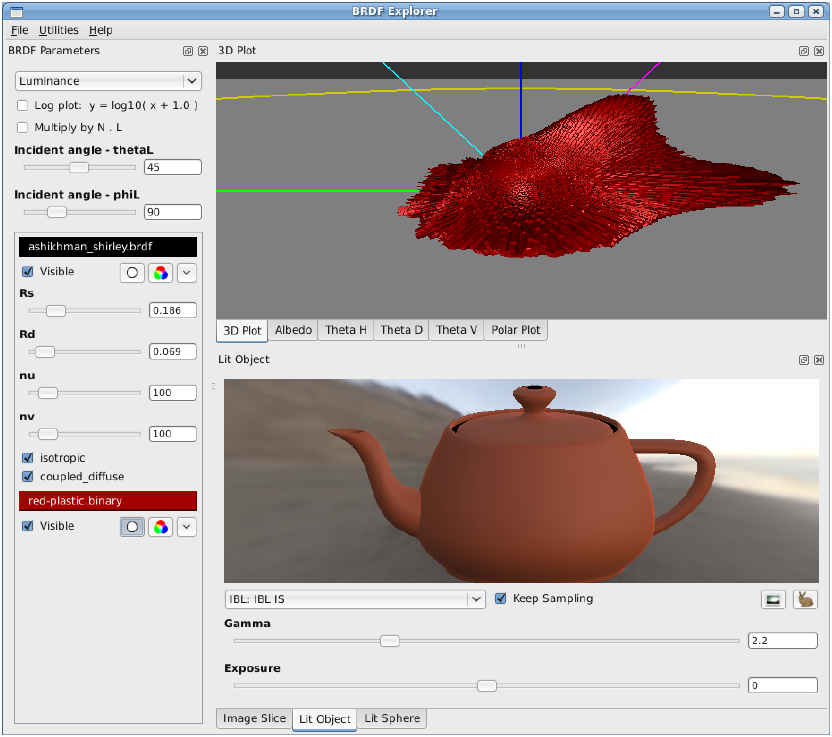
\includegraphics[height=\appH]{Figures/disneyBRDFApp.png}
  \caption[Ukázka aplikace Disney BRDF Explorer]{Ukázka aplikace Disney BRDF Explorer~\cite{DisneyBRDF}}%
  \label{fig:disneyBrdfApp}%
\end{figure}

Článek~\cite{brdfviz} se zabývá implementací systému pro vizualizaci BRDF funkcí dostupných v databázi \textquote{Oregon BRDF Library}\footnote{\url{https://math.nist.gov/~FHunt/appearance/obl.html}}. Je možné vizualizovat i uživatelsky zadané funkce, je potřeba dodržet interní formát definovaný knihovnou Oregon BRDF Library. Samotná vizualizace je interaktivní, je možné za běhu měnit parametry funkcí, přepínat mezi jednotlivými BRDF funkcemi a porovnávat je. Aplikace neumožňuje vizualizovat výsledný render modelu s použitím zvolené BRDF funkce. Aplikace je implementována za pomocí knihovny AVS Express. Výsledná aplikace není veřejně dostupná. Ukázka aplikace je zobrazena na \hyperref[fig:walkerBrdfApp]{obrázku~\ref{fig:walkerBrdfApp}}.\par

\begin{figure}[ht]
  \centering
  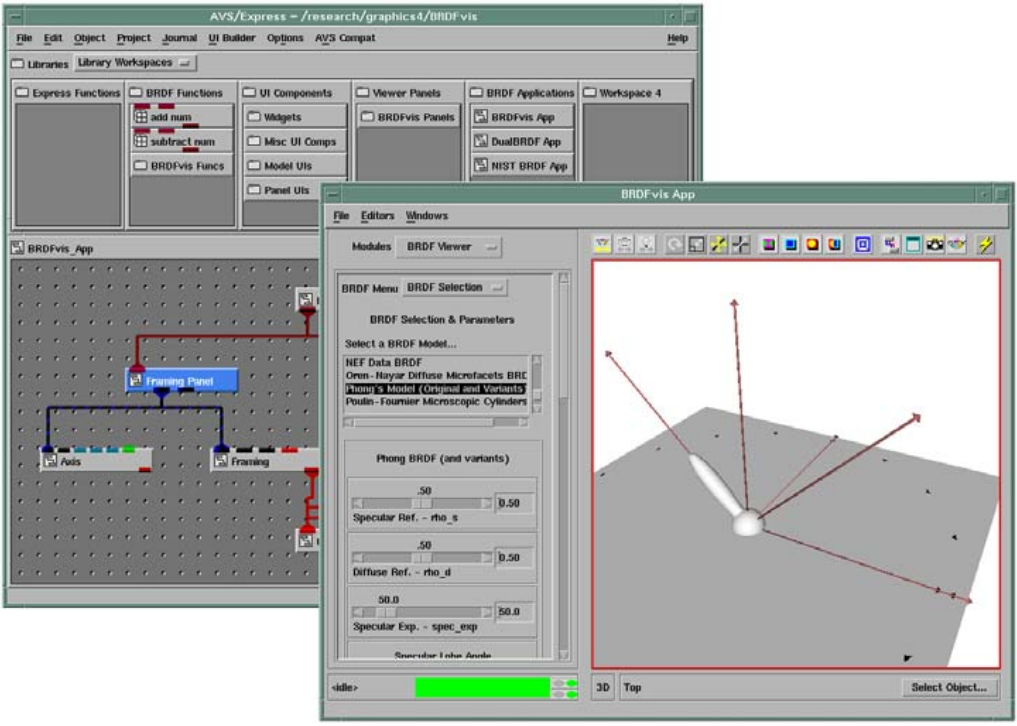
\includegraphics[height=\appH]{Figures/brdfvisWalker.png}
  \caption[Ukázka aplikace BRDFvis]{Ukázka aplikace BRDFvis~\cite{brdfviz}}%
  \label{fig:walkerBrdfApp}%
\end{figure}

Existují také aplikace, které je možné používat v prohlížeči. Taková aplikace je např.\ Photongram\footnote{\url{http://shihchinw.github.io/Photongram}}. Aplikace umožňuje zobrazení čtyř základních BRDF funkcí. Jednotlivým funkcím lze nastavovat parametry, je také možné zobrazit finální render. Není však možné zobrazit finální render i vizualizaci BRDF funkce zároveň. Aplikace má dle mého názoru neintuitivní ovládání. Mezi jednotlivými prvky aplikace je přepínání řešeno pomocí klávesových zkratek, které při prvotním spuštění nejsou nijak představeny. Je možné se k nim dostat pouze pomocí úmyslného kliknutí na tlačítko s nápovědou. Nastavení úhlu vstupního paprsku je realizováno pomocí nastavení na jednotkové kouli. Pouhé použití tohoto způsobu nastavení je nepřesné a neintuitivní. Aplikace je v aktivním vývoji a nefunguje stabilně. Ukázka vizualizace BRDF funkce pomocí aplikace Photongram je zobrazena na \hyperref[fig:photongramApp]{obrázku~\ref{fig:photongramApp}}.\par

\begin{figure}[ht]
  \centering
  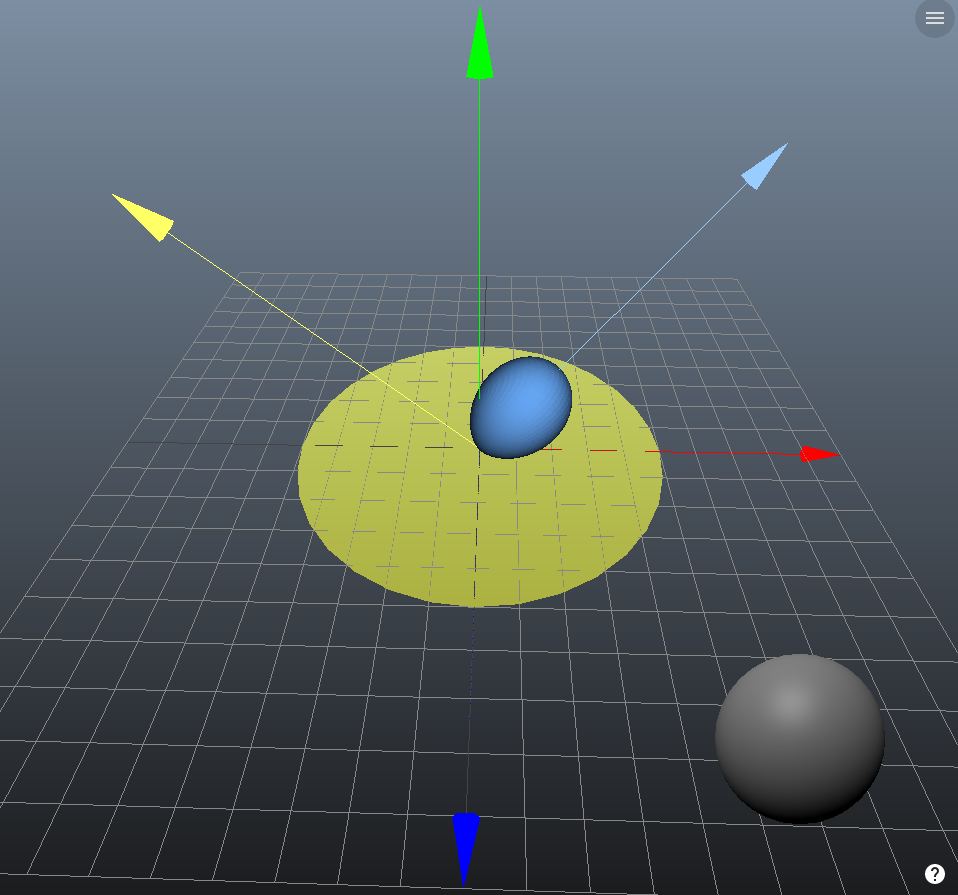
\includegraphics[height=\appH]{Figures/photongram.png}
  \caption[Ukázka aplikace Photongram]{Ukázka aplikace Photongram}%
  \label{fig:photongramApp}%
\end{figure}


Další webovou službou pro vizualizaci BRDF je BSDF Visualizer\footnote{\url{https://n8vm.github.io/BSDF-Visualizer/}}. Aplikace podporuje zobrazení základních BRDF funkcí, větší část zobrazovaných funkcí jsou různé modifikace BRDF podle Disney. Je také možné načíst uživatelsky implementovanou BRDF funkci, definovanou kódem pro GLSL shader. Načtený kód pro BRDF funkci je třeba dodat ve formátu \textquote{yaml}, je možné přidat nejen implementaci BRDF funkce spolu s pomocnými funkcemi, ale i parametry pro funkci ve formátu uniformních proměnných. Aplikace umožňuje také vizualizaci finálního renderu, který může být osvětlen pomocí bodového světla, nebo pomocí sférické mapy. Zajímavou funkcí pak je možnost přímé vizualizace BRDF funkce na povrchu renderovaného tělesa. Ukázka aplikace je zobrazena na \hyperref[fig:bsdfVizApp]{obrázku~\ref{fig:bsdfVizApp}}.

\begin{figure}[ht]
  \centering
  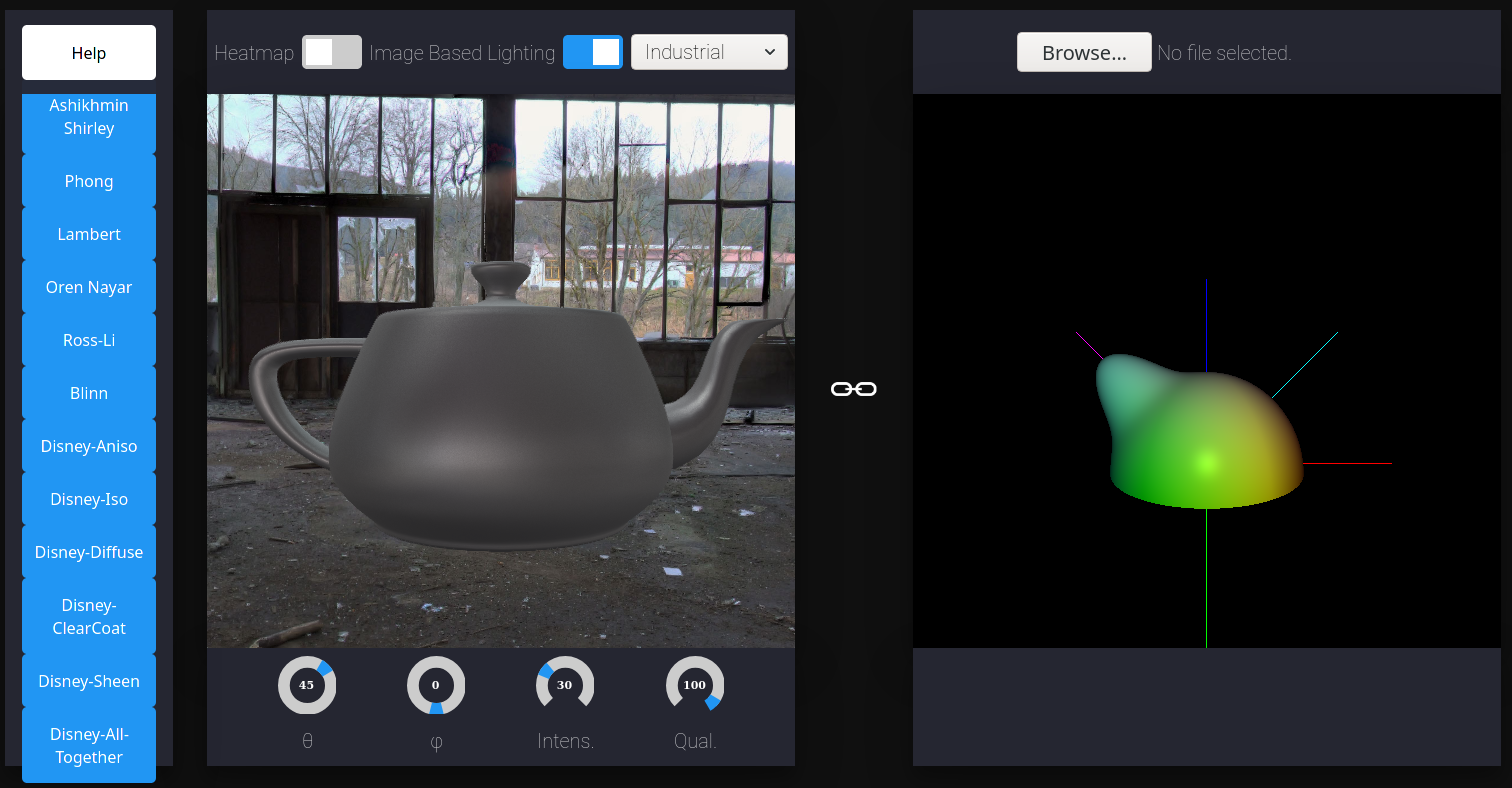
\includegraphics[height=\appH]{Figures/BSDFvisApp.png}
  \caption{Ukázka aplikace BSDF Visualizer}%
  \label{fig:bsdfVizApp}%
\end{figure}

\section{Aplikace pro návrh BRDF funkcí}
Ve článku~\cite{Fors2009BRDFLabAG} je popsána aplikace BRDFLab~\cite{sourceBRDFLab} pro vizualizaci BRDF funkcí zadaných analyticky, pomocí naměřených dat z MERL databáze, nebo pomocí dat získaných simulací. Také je možné vytvořit BRDF funkce kombinací analyticky zadaných, předpřipravených laloků (např. Lambert, Phong\dots). Aplikace také umožňuje vizualizaci finálního renderu s použitím BRDF funkce. Není však možné zobrazit zároveň vizualizaci BRDF funkce a finální render. Zajímavou funkcionalitou je tzv.\ \textquote{fitting} -- možnost aproximace komplexních BRDF funkcí (např.\ z MERL databáze) pomocí kombinace analyticky zadaných modelů. Při načtení naměřených dat Aplikace je distribuována jako open-source, pro GUI je použita knihovna QT, pro rendering je použita knihovna Ogre3D. Ukázka aplikace je zobrazena na \hyperref[fig:brdflabApp]{obrázku~\ref{fig:brdflabApp}}.\par

\begin{figure}[ht]
  \centering
  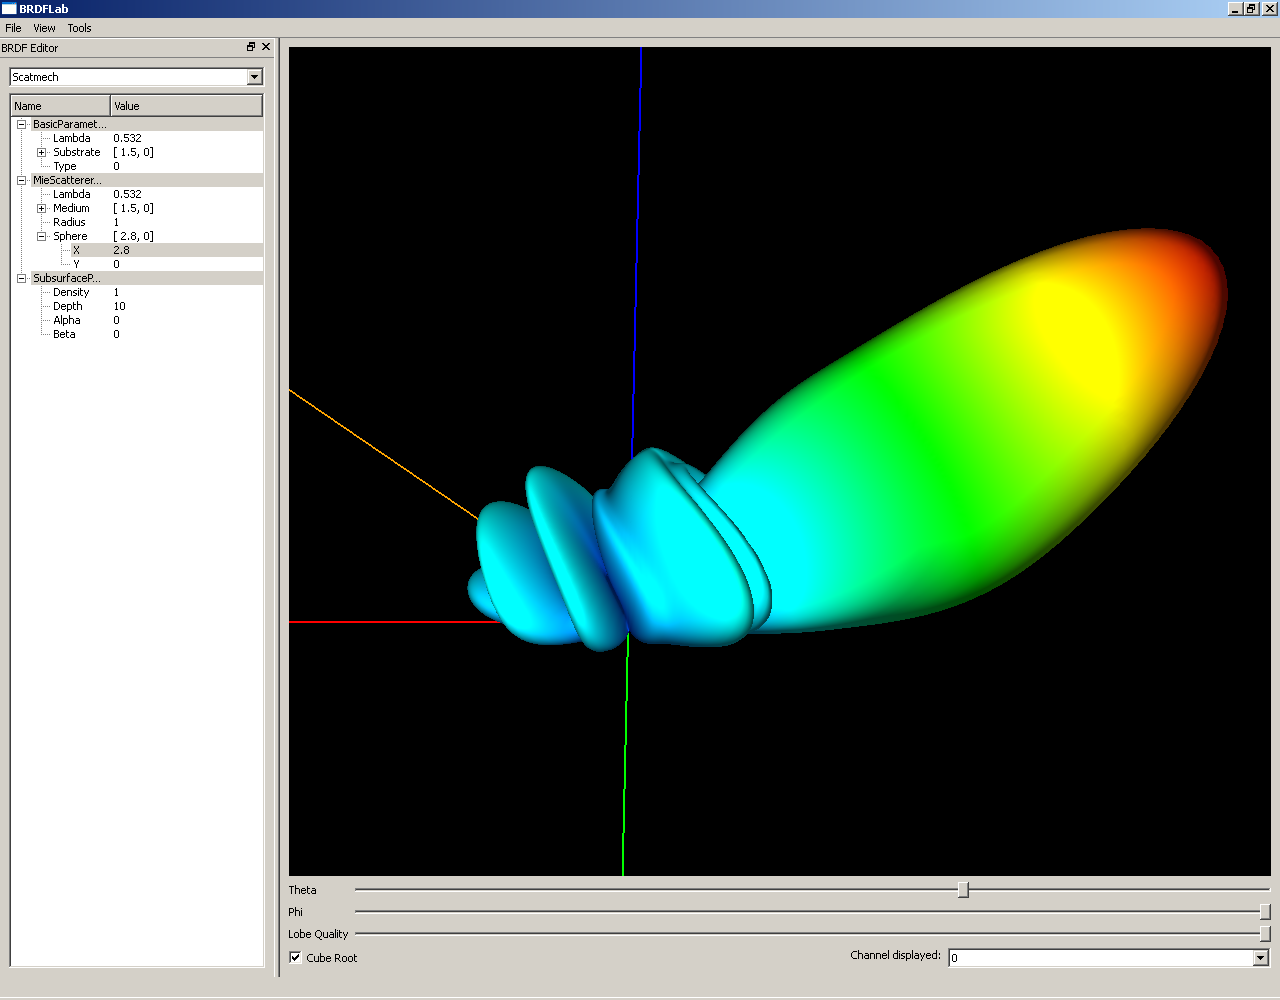
\includegraphics[height=\appH]{Figures/brdflab.png}
  \caption[Ukázka aplikace BRDFLab]{Ukázka aplikace BRDFLab~\cite{Fors2009BRDFLabAG}}%
  \label{fig:brdflabApp}%
\end{figure}

Článek~\cite{brdfshop} se zabývá popisem aplikace BRDF-Shop, která je primárně určena pro návrh BRDF funkcí založených na Wardově BRDF\@. Aplikace jako taková je implementována jako plugin do 3D editoru Autodesk Maya. Aplikace nemá možnost zadání BRDF funkce analyticky, lze pouze vytvářet nové BRDF funkce s odlesky založenými na laloku Wardovy BRDF funkce. Aplikace je primárně určena grafikům pro tvorbu materiálů, není primárně určena pro vizualizaci. Vytvořená BRDF funkce je však standardně vizualizována. Ukázka aplikace je zobrazena na \hyperref[fig:brdflabApp]{obrázku~\ref{fig:brdfshopapp}}.

\begin{figure}[ht]
  \centering
  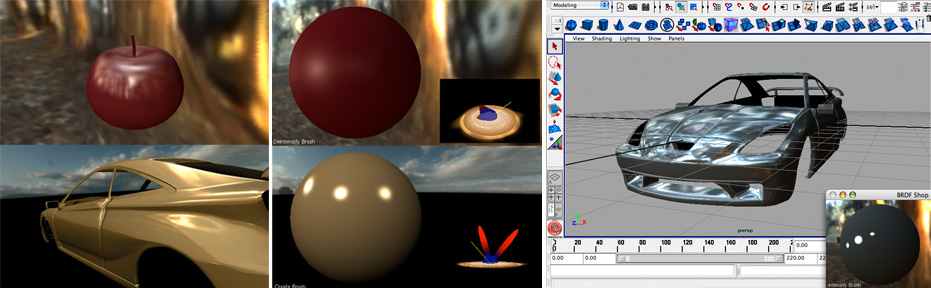
\includegraphics[width=\textwidth]{Figures/BRDFShop.jpg}
  \caption{Ukázka aplikace BRDF-Shop}%
  \label{fig:brdfshopapp}%
\end{figure}

\section{Shrnutí}
Jednotlivé aplikace pro vizualizaci a návrh BRDF funkcí mají z velké části společnou funkcionalitu a liší se hlavně v detailech. Aplikace se zásadně liší podle způsobu použití na aplikace sloužící čistě k vizualizaci BRDF funkcí a aplikace sloužící primárně pro návrh BRDF funkcí. Všechny aplikace v zásadě přistupují k samotné vizualizaci podobně, výsledky vizualizací jsou srovnatelné. Některé aplikace umožňují zobrazení BRDF funkce s interaktivní změnou parametrů zároveň i se zobrazením výsledného renderovaného obrázku. Některé aplikace také umožňují načíst uživatelsky zadané BRDF funkce. Žádná ze zde implementovaných aplikací nenabízí možnost zobrazení vzorkovacích funkcí, které jsou při použití BRDF funkcí důležité.

\section{Požadavky na implementovanou aplikaci}
Implementovaná aplikace by měla mít možnost zobrazení vybraných analyticky zadaných BRDF funkcí. Zobrazení by mělo být interaktivní, měla by být možná změna parametrů jednotlivých funkcí za běhu aplikace. Také by měla být možnost zobrazení renderovaného modelu s použitím aktuálně zadané BRDF funkce s aktuálními parametry. Vykreslování objektu by mělo korespondovat se změnou parametrů, při změně parametrů dojde k překreslení. Objekt by měl být osvětlen pomocí HDR mapy, měla by být dostupná i možnost tzv. \textquote{furnace testu} pro ověření fyzikální korektnosti. Vykreslování modelu by mělo být rychlé, s použitím akceleračních technik. Součástí aplikace by také měla být vizualizace vzorkovacích funkcí.

\clearpage
\chapter{Fotorealistický rendering}
V počítačové grafice existuje odjakživa snaha přiblížit se výsledky reálnému světu. Fotorealistická grafika je taková, která se tváří jako nerozeznatelná např.\ od fotografie. Pro fotorealismus je nutné, aby rendering co nejpřesněji simuloval fyzikální principy šíření světla. Renderingem se rozumí proces výpočtu geometrie, pozice objektů a osvětlení. V roce 1986 byl realistický rendering popsán integrální rovnicí popisující přenos světelné energie ve scéně. Zobrazovací rovnice byla popsána simultánně ve článcích~\cite{KajiyaRenderEq} a~\cite{ImmelRenderEq}. Kajiya v~\cite{KajiyaRenderEq} popisuje různé možnosti řešení integrálu zobrazovací rovnice, mimo jiné i pomocí Monte Carlo metody, kterou pojmenoval jako path tracing~\cite{HainesRayTracingGems2019}. Immel, Cohen a Greenberg v článku~\cite{ImmelRenderEq} navrhují řešení zobrazovací rovnice pomocí metody konečných prvků, kterou pojmenovali jako metodu radiozity. V této práci se budu dále zabývat řešením zobrazovací rovnice pouze pomocí metody Monte Carlo.\par
Zobrazovací rovnici lze vyjádřit \hyperref[eq:render]{vzorcem~\ref{eq:render}}. Zobrazovací rovnice popisuje globální šíření světla ve scéně v ustáleném stavu

\begin{equation} \label{eq:render}
  \outRadiance = \emitRadiance + \int_{H \left( \point \right)}^{~}\radiancert \brdf \inDotNorm \,d\inVec\,.
\end{equation}

Pro popis odrazu světla slouží rovnice odrazu, definovaná \hyperref[eq:render]{vzorcem~\ref{eq:reflect}}. Tuto rovnici je možné použít pro výpočet odražené záře od objektu, pokud je známá zář dopadající na objekt

\begin{equation} \label{eq:reflect}
  \reflRadiance = \int_{H \left( \point \right)}^{~}\inRadiance \brdf \inDotNorm \,d\inVec\,.
\end{equation}

Rovnice odrazu bez BRDF členu a bez emisivního členu vyjadřuje ozáření daného bodu (viz \hyperref[eq:irradiance]{vzorec~\ref{eq:irradiance}})~\cite{Dutre2003GICompendum}

\begin{equation} \label{eq:irradiance}
  \irradiance = \int_{H \left( \point \right)}^{~}\inRadiance \inDotNorm \,d\inVec\,.
\end{equation}

\section{Osvětlení}
Jak už bylo zmíněno, realistický rendering se zabývá co nejpřesnější simulací šíření světla ve scéně. V reálném světě je světlo jako takové elektromagnetické záření. Viditelná část světla odpovídá zhruba intervalu \(\intervaloo{390}{760}nm\) vlnové délky. Při renderingu se často pracuje pouze s geometrickou optikou. Geometrická optika zjednodušuje při šíření světla světelné paprsky na analyticky zadané orientované úsečky, zanedbává vlastnosti vycházející z vlnové podstaty světla. Z pohledu počítačové simulace jsou světelné paprsky vyzařovány světelnými zdroji do scény. Objekty ve scéně se světelnými paprsky interagují (např.~pohlcují, odráží, lámou\dots). Tato interakce objektu a světla definuje, jak výsledný objekt vizuálně působí.\par
Osvětlení objektů ve scéně je popsáno osvětlovacím modelem. Pokud daný osvětlovací model bere v potaz vliv na osvětlení pouze přímými zdroji světla, jedná se o lokální osvětlovací model. Pokud osvětlovací model bere v potaz i světlo odražené ostatními objekty ve scéně, které samy o sobě žádné světlo nevyzařují, jedná se o globální osvětlovací model. Rozdíl mezi osvětlením lokálním a globálním osvětlovacím modelem je patrný z \hyperref[fig:localVsGlobalIllum]{obrázku~\ref{fig:localVsGlobalIllum}}\footnote{Výsledné renderované obrázky byly vytvořeny v programu Blender 2.92}.

\begin{figure}[ht]%
  \centering
  \subfloat[Lokální osvětlovací model]{{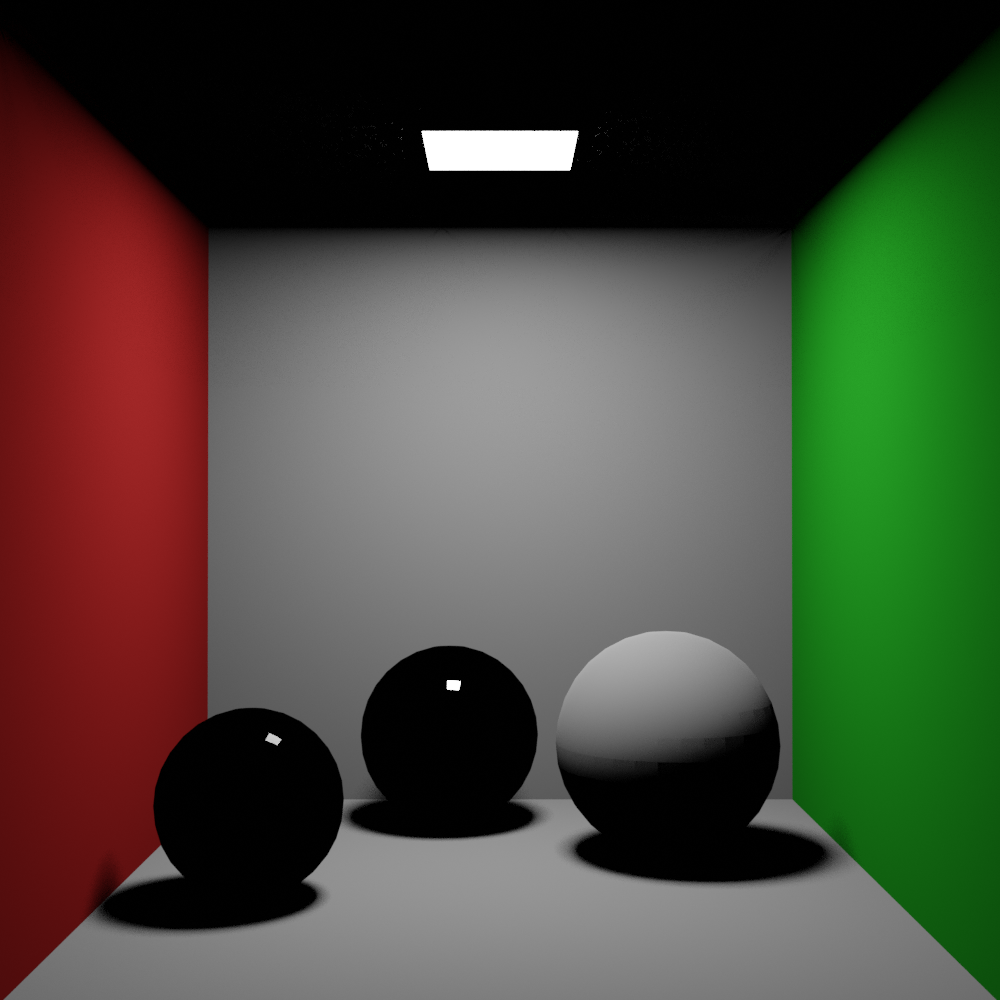
\includegraphics[width=6cm]{Figures/cornelldirect.png} }}%
  \qquad
  \subfloat[Globální osvětlovací model]{{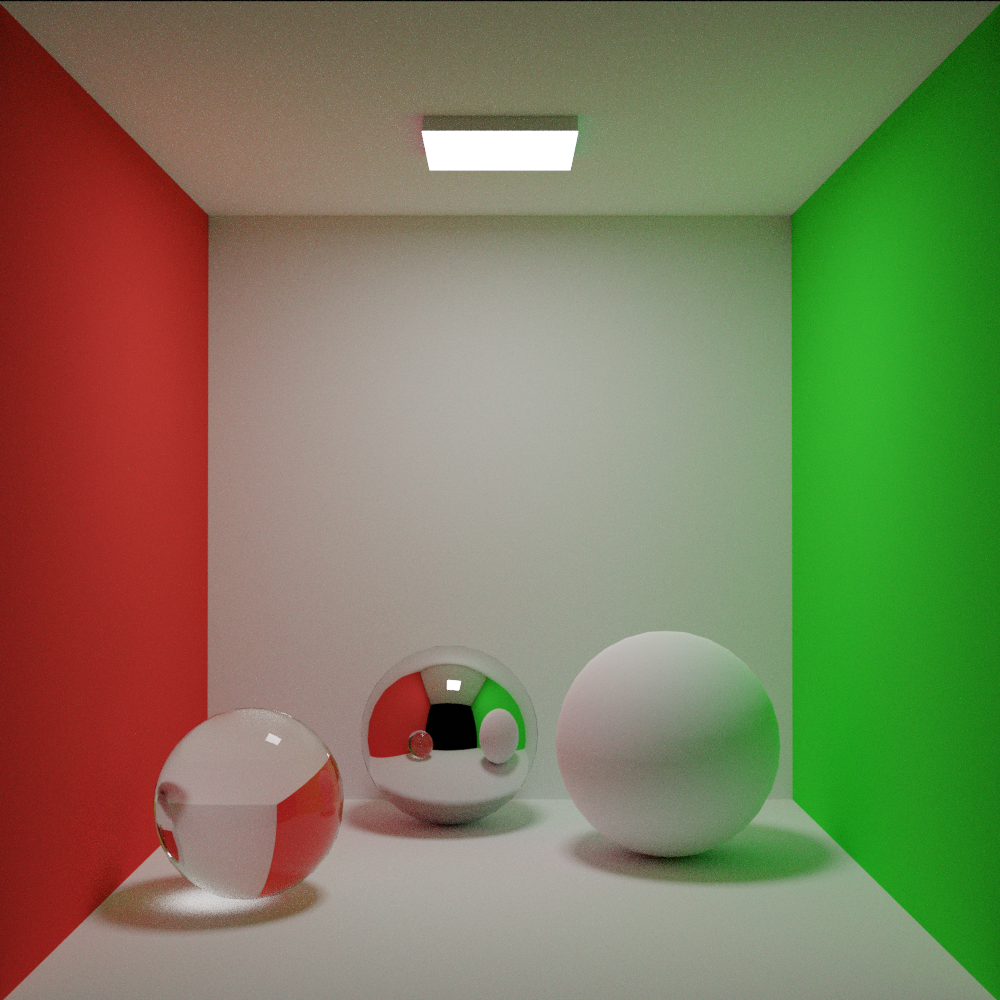
\includegraphics[width=6cm]{Figures/cornellIndirect.png} }}%
  \caption{Srovnání osvětlovacích modelů}%
  \label{fig:localVsGlobalIllum}%
\end{figure}

\subsection{Osvětlení pomocí mapy prostředí}
V počítačové grafice je v zásadě standard použití mapy prostředí jako pozadí pro scénu. Toto použití je pak dále rozšířeno v realistickém renderingu, mapa prostředí pak slouží pro osvětlení. Mapa prostředí pak v zásadě určuje osvětlení jednoho bodu ve scéně okolním prostředím, které je uloženo jako obrazová data. Reprezentace osvětlení z pohledu jednoho bodu je zobrazeno na \hyperref[fig:hdrMapProbe]{obrázku~\ref{fig:hdrMapProbe}}. V praktické implementaci se pak většinou používá sférická mapa (lze se také setkat s pojmem tzv. \textquote{latitude, longitude} mapování), která je aplikována jako textura na pomyslnou kouli obklopující scénu, nebo tzv. \textquote{cube map}, kde je mapa použita jako textura pro pomyslnou krychli obklopující scénu. Ukázka sférické mapy je zobrazena na \hyperref[fig:hdrMapSpheric]{obrázku~\ref{fig:hdrMapSpheric}}, ukázka cube map je ukázána na \hyperref[fig:hdrMapCube]{obrázku~\ref{fig:hdrMapCube}}. Sférická mapa je častěji používána s technologií ray tracing, z důvodu jednoduššího převodu směrového vektoru sledovaného paprsku do sférických souřadnic a následně do samotného texelu této textury. Cube map je pak častěji používána v klasické rasterizaci z důvodu jednoduchého použití díky přímé podpoře v OpenGL shaderech.\par
Fotorealistického osvětlení modelů ve scéně pomocí mapy prostředí je dosaženo díky odrazům paprsků od povrchu objektů, které jsou odraženy do mapy prostředí. Texely mapy prostředí tak mají přímý vliv na osvětlení objektu a není potřeba použít ve scéně bodová světla. Pro fotorealismus je také důležitý formát mapy prostředí. Standardní fotografie nemají dostatečnou bitovou hloubku pro zachycení reálné intenzity světla. Je proto vhodné použít HDR snímky, kde jsou hodnoty jednotlivých pixelů reprezentovány jako reálná čísla ve formátu float.

\begin{figure}[ht]%
  \centering
  \subfloat[\label{fig:hdrMapProbe}]{{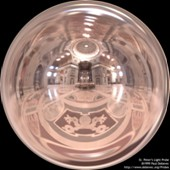
\includegraphics[height=3cm]{Figures/mapProbe.jpg}}}%
  \qquad
  \subfloat[\label{fig:hdrMapSpheric}]{{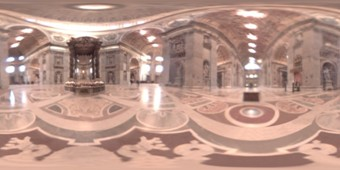
\includegraphics[height=3cm]{Figures/mapSphere.jpg}}}%
  \qquad
  \subfloat[\label{fig:hdrMapCube}]{{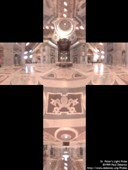
\includegraphics[height=3cm]{Figures/mapCube.jpg}}}%
  \caption[Ukázka různých map prostředí]{Ukázka různých map prostředí~\cite{DebevecIBL}}%
  \label{fig:hdrMapsComparison}%
\end{figure}

\section{Rendering pomocí metody sledování paprsku}
Při renderingu pomocí klasických metod se postupuje pomocí standardního zobrazovacího řetězce. Postup je ve zkratce následující: Vrcholy tělesa jsou nahrány do GPU, následně se ve fragment shaderu aplikují transformační matice a matice pro převod z lokálního do globálního prostoru. Následně je provedena rasterizace tělesa. Nakonec je ve fragment shaderu vypočítáno osvětlení tělesa. Standardní zobrazovací řetězec má tu výhodu, že je možné renderovat za běhu programu, v reálném čase. Nevýhodou je však ztráta jisté reálnosti výstupu.\par
Při použití metody sledování paprsku je perspektivní promítání realizováno pomocí sady přímek (paprsků). Paprsky jsou konstruovány takovým způsobem, že procházejí středem promítání. Směry těchto přímek pak korespondují s rozmístěním jednotlivých pixelů generovaného obrazu na pomyslné promítací rovině. Následně se provádí traverzace ve scéně (hledání objektu ve scéně, který byl protnut paprskem). Při protnutí tělesa je možné následně počítat další odrazy paprsků a simulovat tak šíření světla ve scéně. Výhodou použití metody sledování paprsků je možnost velmi reálných výsledků. Nevýhodou je ale vysoká výpočetní náročnost. Výpočet komplexních scén pouze pomocí metod sledování paprsků v reálném čase je komplikovaný problém. V současné době je možná hardwarová akcelerace na grafických kartách. Pro urychlení výpočtu jsou také používány hluboké neuronové sítě (např.\ technologie Nvidia DLSS). Je možné provádět výpočet pro nižší rozlišení a následně provést upscaling (zvýšení rozlišení). Neuronová síť je schopná dopočítat chybějící data. Výsledkem je dle Nvidia obraz svou kvalitou srovnatelný s výpočtem ve vyšším rozlišení bez použití této technologie.

\section{Řešení zobrazovací rovnice}
Zobrazovací rovnice má formu integrálu, který se počítá přes pomyslnou polokouli vytvořenou nad bodem, orientovanou podél normály bodu. Na výslednou hodnotu má vliv nekonečné množství příchozích paprsků ze všech směrů na povrchu polokoule. Zář \(\inRadiance\) dopadající na bod mohlo být odraženo jiným bodem ve scéně. Z toho vyplývá, že výpočet osvětlení je nekonečně rekurzivní. Korektní analytické řešení zobrazovací rovnice z toho důvodu není možné. Z matematického hlediska existuje více způsobů, jak řešit integrály. Metoda Monte Carlo se opírá o princip z teorie pravděpodobnosti a matematické statistiky, že průměr velkého počtu náhodných veličin se přiblíží střední hodnotě. Řešení zobrazovací rovnice pomocí metody Monte Carlo navrhuje Kajiya v~\cite{KajiyaRenderEq}.\par
Monte Carlo je stochastická metoda, v matematice často využívaná pro řešení složitějších integrálů. Metoda Monte Carlo řeší integrály modelováním náhodných veličin a následným odhadem jejich charakteristik. Nejčastěji tato metoda modeluje náhodné veličiny tak, že se střední hodnota rovná hledané hodnotě~\cite{MonteCarlo}.\par
Pro řešení zobrazovací rovnice jsou typicky generovány náhodné směry odrazu světla. Výsledný obraz je poté tvořen průměrem určitého počtu vzorků. Typicky se u výsledných obrázků vytvořených pomocí metody path tracing uvádí počet vzorků na pixel. Se zvyšujícím se počtem vzorků na pixel typicky stoupá ostrost a přesnost výsledného obrazu. S nízkým počtem vzorků je typicky obraz zatížen šumem (viz srovnání na \hyperref[fig:samplesPpxComparison]{obrázku~\ref{fig:samplesPpxComparison}})\footnote{Výsledné renderované obrázky byly vytvořeny v programu Blender 2.92}.

\begin{figure}[ht]%
  \centering
  \subfloat[1 vzorek na pixel]{{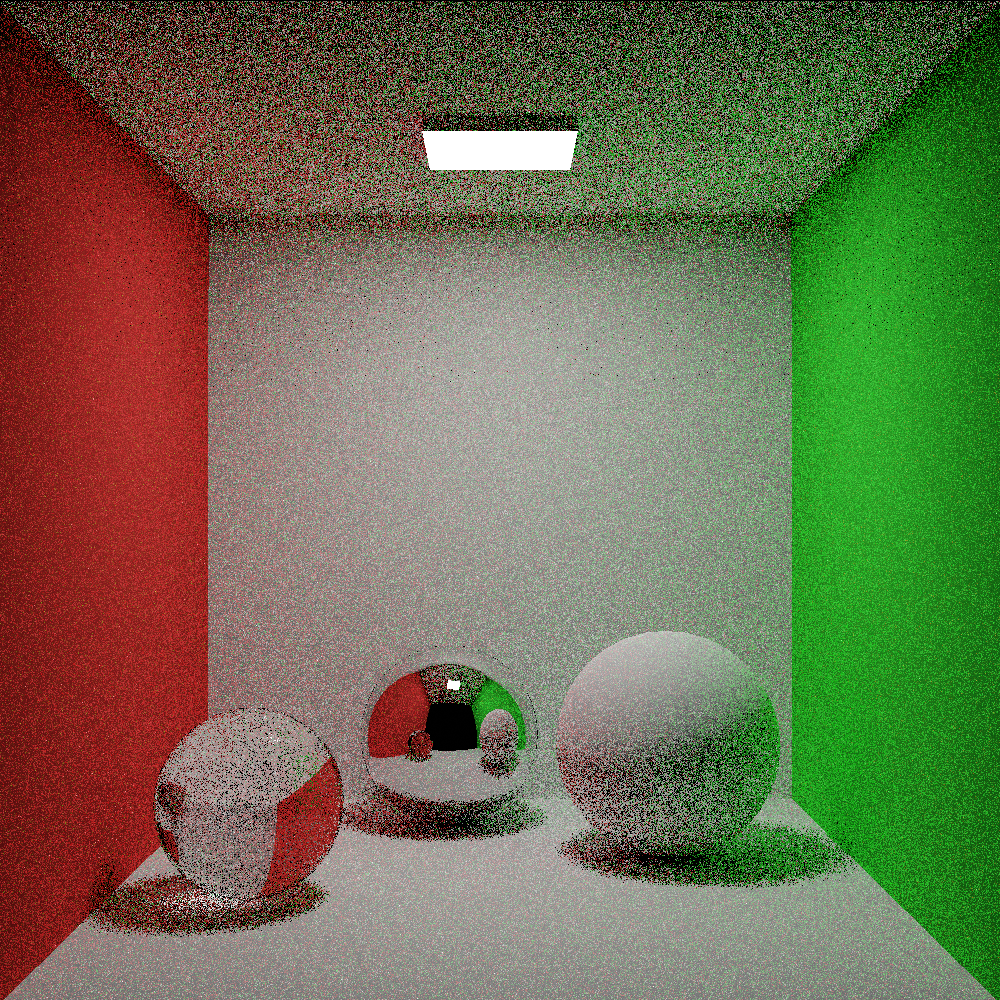
\includegraphics[width=6cm]{Figures/cornell1ppx.png} }}%
  \qquad
  \subfloat[4 vzorky na pixel]{{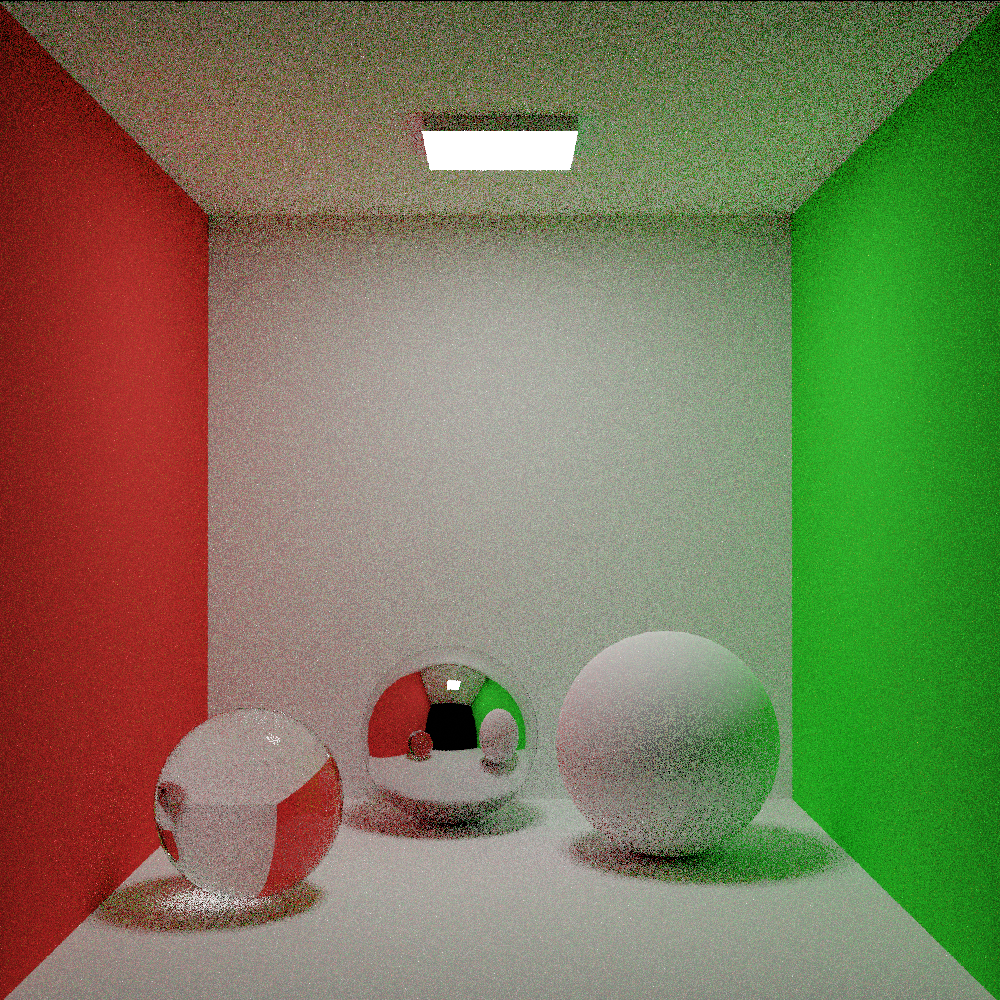
\includegraphics[width=6cm]{Figures/cornell4ppx.png} }}%
  \qquad
  \subfloat[16 vzorků na pixel]{{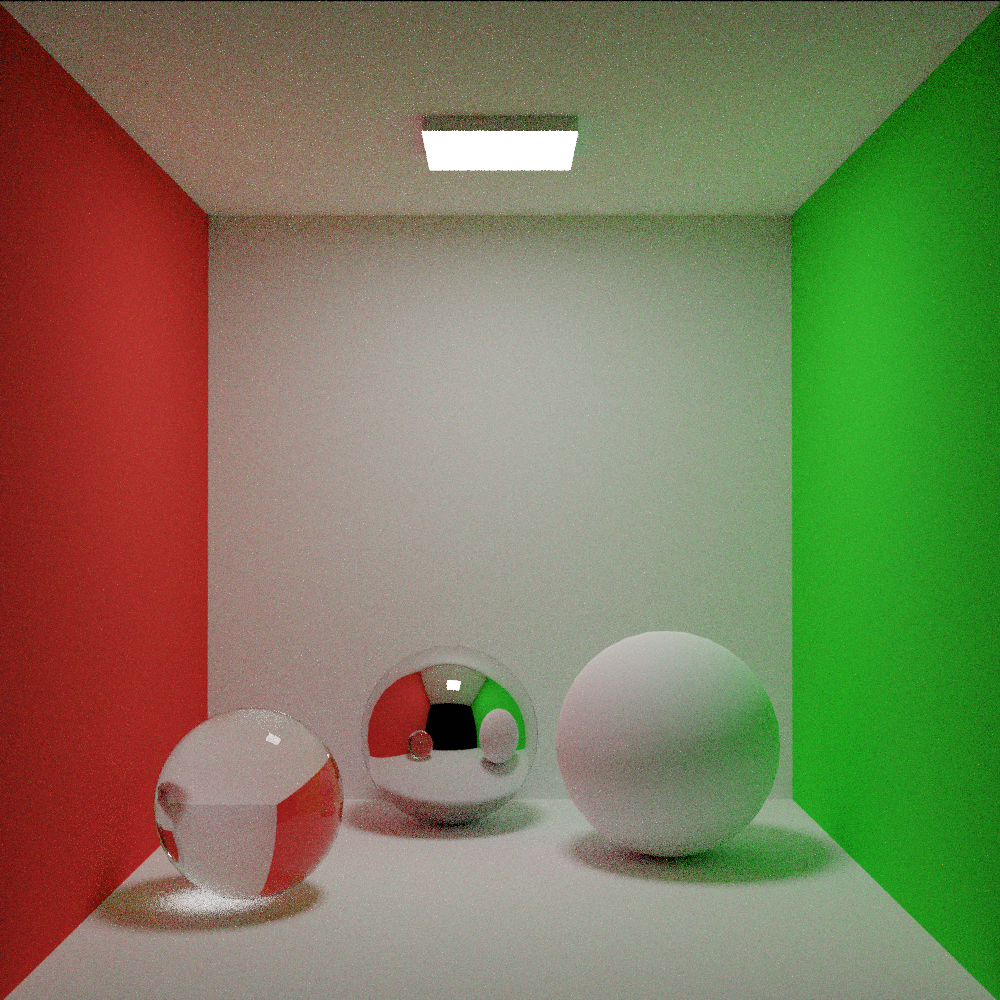
\includegraphics[width=6cm]{Figures/cornell16ppx.png} }}%
  \qquad
  \subfloat[64 vzorků na pixel]{{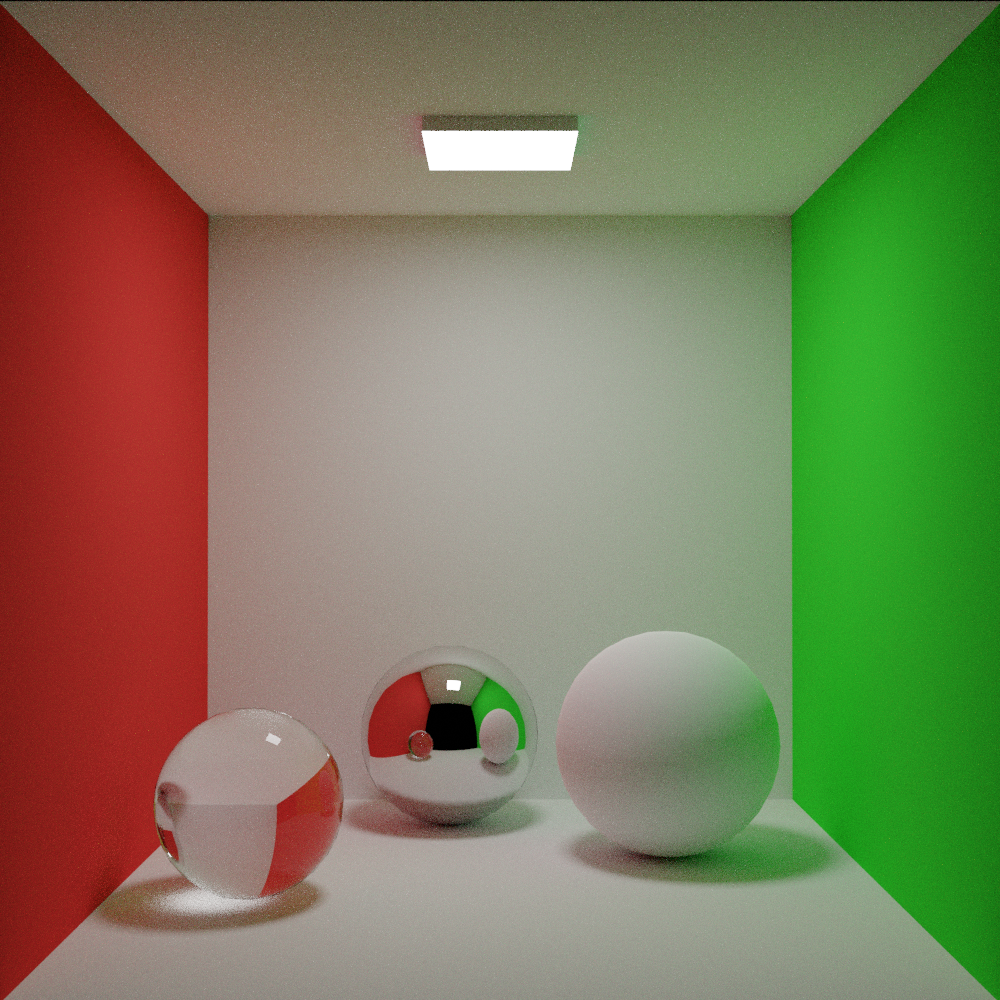
\includegraphics[width=6cm]{Figures/cornell64ppx.png} }}%
  \caption[Srovnání výsledných obrázků podle počtu vzorků na pixel]{Srovnání výsledných obrázků podle počtu vzorků na pixel. S vyšším počtem vzorků na pixel se dramaticky snižuje šum.}%
  \label{fig:samplesPpxComparison}%
\end{figure}



\clearpage
\chapter{BRDF}
BRDF je matematická funkce, která definuje pro daný materiál odrazivost povrchu. Určuje pro každý bod tělesa distribuci odrazu světla. Na \hyperref[fig:brdf2D]{obrázku~\ref{fig:brdf2D}} je znázorněn základní princip BRDF funkce. Vektor \(\normVec\) je normála povrchu, \(\inVec\) značí směr ke světelnému zdroji, \(\outVec\) značí směr k pozorovateli (ke kameře). BRDF je definována pro dvojici vektorů  \(\inVec\) a \(\outVec\) v daném bodě \(p\) pomocí \hyperref[eq:brdf]{vzorce~\ref{eq:brdf}}
% Pbrt strana 350

\begin{equation} \label{eq:brdf}
  \brdf = \frac{d\outRadiance}{\difirradiance} = \frac{d\outRadiance}{\inRadiance \inDotNorm d\inVec}\,.
\end{equation}

Je žádoucí, aby BRDF funkce splňovaly některá základní pravidla. Je důležitá fyzikální přesnost BRDF funkce, pro kterou musí být splněny následující podmínky~\cite{PHARR2017313}:

\begin{itemize}
  % 10.3 Reciprocity 
  \item Princip vzájemnosti (Helmholtzův princip reciprocity,~\cite{hapke_2012}) -- Pro všechny dvojice \(\inVec\) a \(\outVec\) platí: \(\brdf = f_r\left(p,\inVec,\outVec\right)\).
  \item Princip zachování energie -- Celková energie odraženého světla nemůže být vyšší než energie příchozího světla. Zároveň je také žádoucí, aby bylo odraženo a pohlceno všechno příchozí světlo.
  \item BRDF musí mít vždy nezáporný výsledek.
\end{itemize}
Tyto podmínky jsou potřeba pro korektní výstup BRDF funkce a je možné je považovat za základní trojici podmínek. Dále je možné definovat několik dalších podmínek pro BRDF funkce, aby výsledné rendery byly věrohodné z vizuálního hlediska~\cite{EnergyConservingRadziszewski}:

\begin{itemize}
  \item BRDF funkce by měla být spojitá. Nespojitosti jsou pro lidské oko nepřirozené. Spojitost BRDF funkcí mohou porušovat např. BRDF funkce, které využívají metody \textquote{min}, \textquote{max}.
  \item BRDF funkce by měla mít možnost nastavení parametru zrcadlové složky tak, aby bylo možné dosáhnout i matného povrchu.
  \item BRDF funkce by měla mít možnost nastavení parametru zrcadlové složky tak, že pokud je hodnota tohoto parametru \(1\), BRDF funkce se blíží ideálnímu odrazu.
  \item Možnost jednoduchého vzorkování -- BRDF funkce by měla být jednoduše vzorkovatelná, pdf funkce pro BRDF funkci by měla být analyticky vyjádřitelná.
\end{itemize}

Další doplňující podmínky lze definovat pro BRDF funkce, které využívají mikroplošky. Podmínky pro BRDF využívající mikroplošky jsou podrobněji rozvedeny v \hyperref[sec:torrancesparrow]{kapitole~\ref{sec:torrancesparrow} Torrance-Sparrow}.

\begin{figure}[ht!]
  \centering
  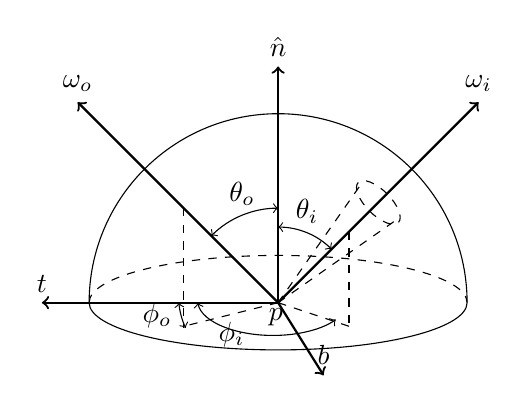
\begin{tikzpicture}[scale=0.6]
    % base circle
    \draw (-4,0) arc (180:360:4 and 1);
    \draw [dashed] (-4,0) arc (180:0:4 and 1);
    % hemisphere
    \draw (-4,0) arc (180:0:4 and 4);

    \draw [thick, ->] (0,0) -- ++(-5,0) node [at end, above] () {\(\vv{t}\)};
    \draw [thick, ->] (0,0) -- ++(135:6cm) node [at end, above] () {\(\outVec\)};
    % y
    \draw [thick, thick, ->] (0,0) -- ++(0,5) node [at end, above] () {\(\normVec\)};
    % z
    \draw [thick, ->] (0,0,0) -- ++(0,-2.5,-2.5) node [at end, above] () {\(\vv{b}\)};
    % lines spanning angle alpha
    \draw [thick, ->] (0,0) -- ++(45:6cm) node [at end, above] () {\(\inVec\)};

    \draw [thin, dashed] (0,0) -- ++(55:3cm);
    \draw [thin, dashed] (0,0) -- ++(35:3cm);

    \draw[thin, dashed, rotate=45] (3,0) ellipse (0.26cm and 0.6cm);

    \draw [thin, <->] (0,0) ++(90:1.6cm) arc (90:45:1.6cm) node [midway, above] () {\(\theta_i \)};

    \draw [thin, dashed] (1.5,1.5) -- ++(0,-2);
    \draw [thin, dashed] (0,0) -- ++(1.5,-0.5);

    \draw [thin, dashed] (-2,2) -- ++(0,-2.53);
    \draw [thin, dashed] (0,0) -- ++(-2,-0.5);

    \draw [thin, <->] (0,0) ++(180:2.1cm) arc (185:205:1.6cm) node [midway, left] () {\(\phi_o\)};

    \draw [thin, <->] (0,0) ++(180:1.7cm) arc (185:326:1.6cm and 0.76cm) node [midway, left] () {\(\phi_i \)};

    \draw [thin, <->] (0,0) ++(90:2cm) arc (90:135:2cm) node [midway, above] () {\(\theta_o\)};


    \draw (-0.05,-0.3) node () {\(p\)};
  \end{tikzpicture}
  \caption{Základní vizualizace BRDF funkce}
  \label{fig:brdf2D}
\end{figure}

\section{Variace BRDF funkcí}
Kromě BRDF funkcí jsou v počítačové grafice definovány i další funkce, které se používají pro popis odrazu světla. BTDF funkce (Bidirectional Transmittance Distribution Function) je distribuční funkce lomu světla, která popisuje průchod světla objektem. BTDF funkce je v zásadě funkce \(\btdf\), pro kterou platí, že vektory \(\inVec\) a \(\outVec\) směřují každý do opačné hemisféry bodu \(\point\).\par
BSDF funkce (Bidirectional scattering distribution function) vzniká v zásadě spojením BRDF a BDTF funkce a popisuje rozptyl světla při kontaktu s objektem.\par
Pokročilejší funkcí je tzv.\ BSSRDF funkce (Bidirectional sub-surface scattering reflectance distribution function). BRDF funkce odráží příchozí světlo vždy ve stejném bodě, BSSRDF funkce modeluje průchod světla a odrazy pod povrchem tělesa. Princip a výpočet BSSRDF funkcí je netriviální, ale použití výsledné funkce má pozitivní dopad na výslednou realističnost scény. Ukázka odrazu světla pomocí BSSRDF funkce je zobrazena na \hyperref[fig:bssrdf]{obrázku~\ref{fig:bssrdf}}.

\begin{figure}[ht]
  \centering
  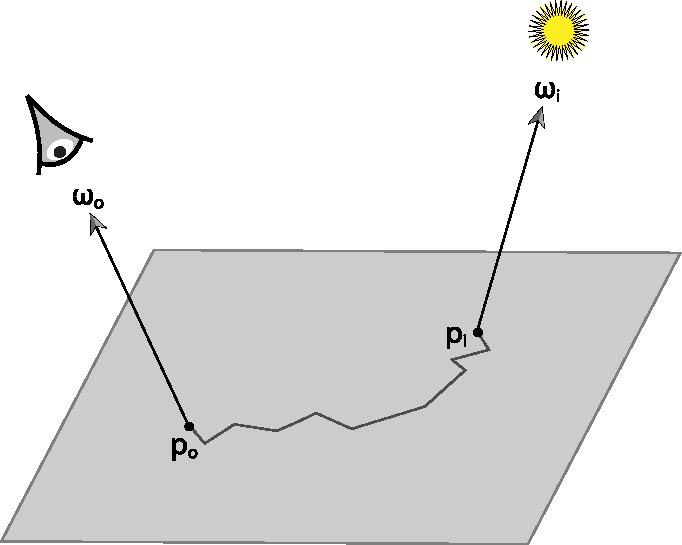
\includegraphics[width=6cm]{Figures/BSSRDF.pdf}%
  \caption[Ukázka principu BSSRDF funkce]{Ukázka principu BSSRDF funkce~\cite{PHARR2017313}}
  \label{fig:bssrdf}
\end{figure}

\section{Přehled BRDF funkcí}\label{sec:brdffunctions}
Následující odstavce se zabývají detailním popisem a vlastnostmi jednotlivých BRDF funkcí. Budou zde vyjmenovány pouze ty BRDF funkce, které byly implementovány v praktické části této diplomové práce. \\
Pro rychlý přehled vlastností jednotlivých BRDF funkcí je možné využít \hyperref[tab:brdfProperties]{tabulku~\ref{tab:brdfProperties}} (převzato z~\cite{BRDFOverview}, zkráceno, doplněno).

\begin{table}[ht]
  \centering
  \begin{tabular}{lcccccrl}
    \toprule
    BRDF model           & \rotatebox{90}{Physical} & \rotatebox{90}{Plausible} & \rotatebox{90}{Fresnel Eq}. & \rotatebox{90}{Anisotropic} & \rotatebox{90}{Sampling} & \rotatebox{90}{Rel.\ cost (cycles)} & Material type         \\
    \midrule
    Ideal reflection     & \true                    & \true                     & \false                      & \false                      & \true                    & \(1\)                               & Mirror, perfect spec. \\
    Lambert              & \true                    & \true                     & \false                      & \false                      & \true                    & \(1\)                               & Perfect diffuse       \\
    Phong                & \false                   & \false                    & \false                      & \false                      & \true                    & \undecided                          & Rough surf.           \\
    Blinn-Phong          & \false                   & \false                    & \false                      & \false                      & \true                    & \(9{,}18\)                          & Rough surf.           \\
    Phys.\ correct Phong & \false                   & \true                     & \false                      & \false                      & \true                    & \undecided                          & Rough surf.           \\
    Torrance-Sparrow     & \true                    & \false                    & \true                       & \true                       & \false                   & \undecided                          & Rough surf.           \\
    Cook-Torrance        & \true                    & \true                     & \true                       & \false                      & \false                   & \(16{,}90\)                         & Metal, plastic        \\
    Oren-Nayar           & \true                    & \true                     & \false                      & \false                      & \true                    & \(10{,}98\)                         & Matte, dirty          \\
    \bottomrule
  \end{tabular}
  \caption[Stručný přehled implementovaných BRDF funkcí]{Stručný přehled implementovaných BRDF funkcí~\cite{BRDFOverview}}
  \label{tab:brdfProperties}
\end{table}

\subsection{Lambert} \label{sec:Lambert}
BRDF podle Beer-Lambertova zákona se řadí mezi analytické modely BRDF\@. Popisuje ideálně matné povrchy, které odráží příchozí světlo do všech směrů rovnoměrně se stejnou pravděpodobností, nehledě na příchozí směr paprsku. Jedná se o nejjednodušší BRDF funkci, je definována \hyperref[eq:lambertBRDF]{vztahem~\ref{eq:lambertBRDF}}~\cite{Koppal2014}
%COmputer vision reference guide katushi, page 675 - Lambertian Reflectance
\begin{equation} \label{eq:lambertBRDF}
  \brdf = \frac{\alb}{\pi} = \text{konstantní}\,.
\end{equation}
Parametr \(\alb\) ve \hyperref[eq:lambertBRDF]{vztahu~\ref{eq:lambertBRDF}} vyjadřuje poměr mezi pohlceným a odraženým světlem. Tato veličina je také odborně nazývána pojmem albedo. Dělení konstantou \(\pi\) zajišťuje platnost zákona zachování energie. Díky nezávislosti na směru vstupního paprsku je také splněna reciprocita. Ukázka vizualizace je zobrazena na \hyperref[fig:lambertBRDFRender]{obrázku~\ref{fig:lambertBRDFRender}} s parametrem \(\alb = 0{,}8\).

\begin{figure}[ht]%
  \centering
  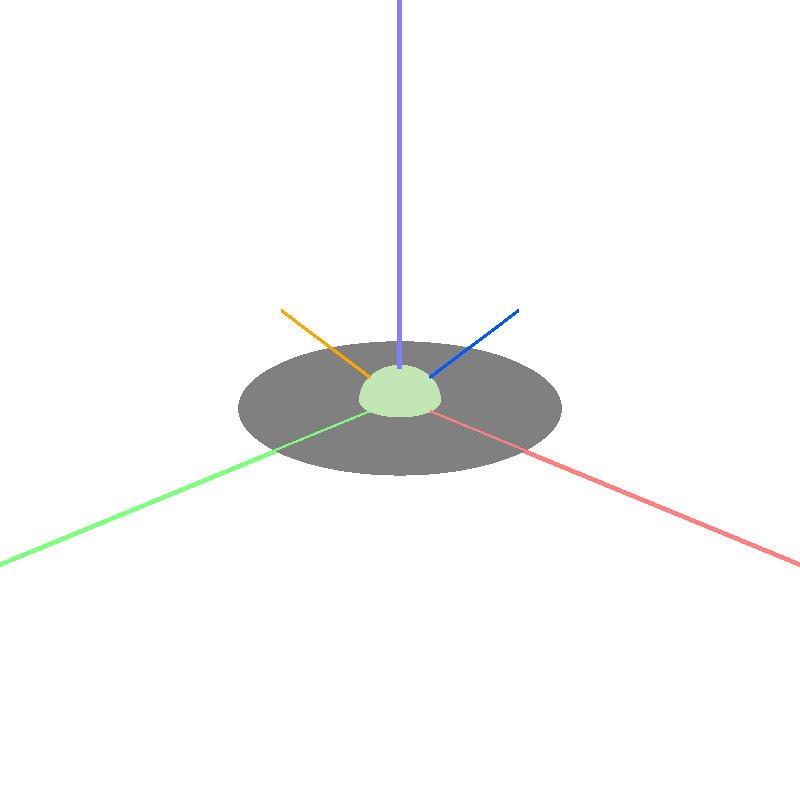
\includegraphics[width=6cm]{Figures/visualizations/brdfLambert.png}%
  \caption{Vizualizace BRDF podle Beer-Lambertova zákona}%
  \label{fig:lambertBRDFRender}%
\end{figure}

\subsection{Ideální odraz} \label{sec:idealReflection}
BRDF pro ideální odraz odráží světlo pouze v jednom směru podle zákona odrazu světla. BRDF funkce pro ideální odraz je definována jako Diracova \(\delta\)-funkce, viz \hyperref[eq:idealReflectionBRDF]{vzorec \ref{eq:idealReflectionBRDF}}. Výsledkem je poté zrcadlový materiál. Ukázka vizualizace je zobrazena na \hyperref[fig:idealReflectionBRDFViz]{obrázku~\ref{fig:idealReflectionBRDFViz}}.


\begin{equation} \label{eq:idealReflectionBRDF}
  \brdf  =  \left\{\begin{matrix*}[l] \infty & \theta_i = \theta_o \\ 0 & \theta_i \neq \theta_o \end{matrix*}\right. = \frac{\delta\left(\cos\theta_i-\cos\theta_o\right)\delta\left(\phi_i-\phi_o+\pi\right)}{\cos\theta_i}
\end{equation}


\begin{figure}[ht]%
  \centering
  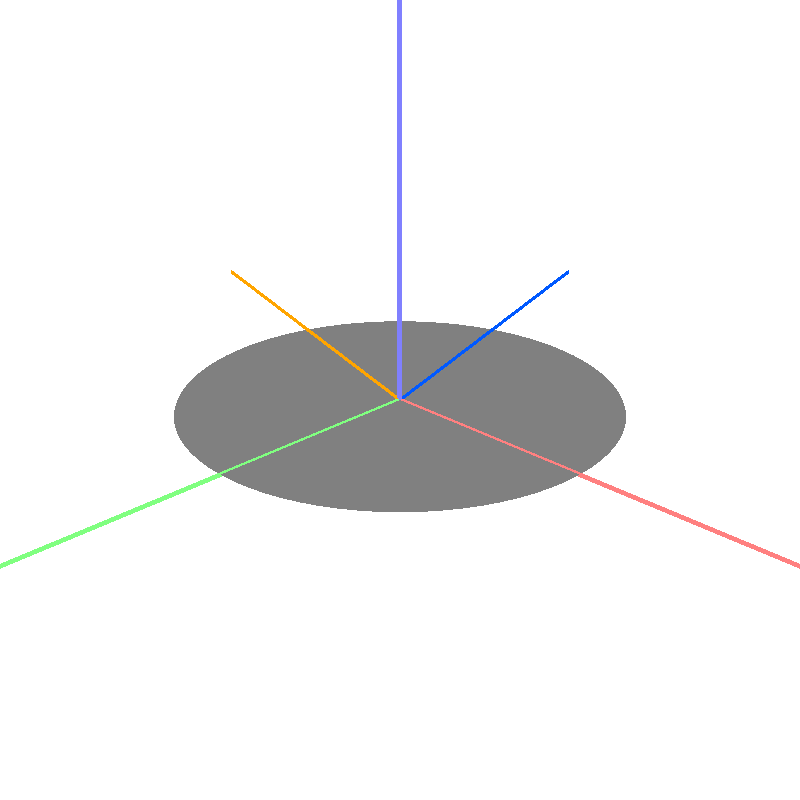
\includegraphics[width=6cm]{Figures/visualizations/brdfMirror.png}
  \caption{Vizualizace BRDF ideálního odrazu}%
  \label{fig:idealReflectionBRDFViz}%
\end{figure}


\subsection{Phong} \label{sec:Phong}
BRDF podle Phongova modelu vychází z Phongova osvětlovacího modelu, řadí se mezi analytické modely BRDF a používá se pro lesklé povrchy. Původní model je definován \hyperref[eq:phongBRDF]{vzorcem~\ref{eq:phongBRDF}}~\cite{Phong1975}. Ukázka vizualizace je zobrazena na \hyperref[fig:phongBRDFRender]{obrázku~\ref{fig:phongBRDFRender}} s parametrem \(n = 32\)
\begin{equation} \label{eq:phongBRDF}
  \brdf = k_s{(\refl\cdot\outVec)}^{n}\,.
\end{equation}

Upravený, také často využívaný Blinn-Phong model, je definován \hyperref[eq:blinnBRDF]{vzorcem~\ref{eq:blinnBRDF}}~\cite{BlinnPhong1977}. Výhodou upraveného Blinn-Phongova modelu oproti klasickému Phongovu modelu je hladší přechod odlesku světla. Ukázka vizualizace je zobrazena na \hyperref[fig:blinnPhongBRDFRender]{obrázku~\ref{fig:blinnPhongBRDFRender}} s parametrem \(n = 32\)

\begin{equation} \label{eq:blinnBRDF}
  \brdf = k_s{(\normVec\cdot\halfVec)}^{n}\,.
\end{equation}

Jak Phong, tak Blinn-Phong modely nejsou fyzikálně přesné -- nesplňují zákon zachování energie, ani zákon reciprocity~\cite{BRDFOverview}. BRDF podle Phongova modelu je možné dále upravit, aby byly splněny pravidla pro fyzikální korektnost. Fyzikálně korektní BRDF podle Phongova modelu je definováno \hyperref[eq:phongPhysicalBRDF]{vzorcem~\ref{eq:phongPhysicalBRDF}}. Pro splnění podmínky zachování energie této varianty je potřeba dodržet \(k_d + k_s \leq 1\)~\cite{LaFortunePhongBRDF}. Tato varianta je stále empirická a fyzikálně korektní je pouze při kolmém pohledu na plošku, pro ostatní směry je výsledná energie nižší. Ukázka vizualizace je zobrazena na \hyperref[fig:physCorrectPhongBRDFRender]{obrázku~\ref{fig:physCorrectPhongBRDFRender}} s parametry \(n = 32, ~k_s = 0{,}1,~k_d = 0{,}8\)

\begin{equation} \label{eq:phongPhysicalBRDF}
  \brdf = \frac{k_d}{\pi} +
  \frac{k_s\left(n+2\right)}{2\pi}{\left(\cos\theta_r\right)}^{n}\,.
\end{equation}

\begin{figure}[ht]%
  \centering
  \subfloat[Vizualizace Phong BRDF\label{fig:phongBRDFRender}]{{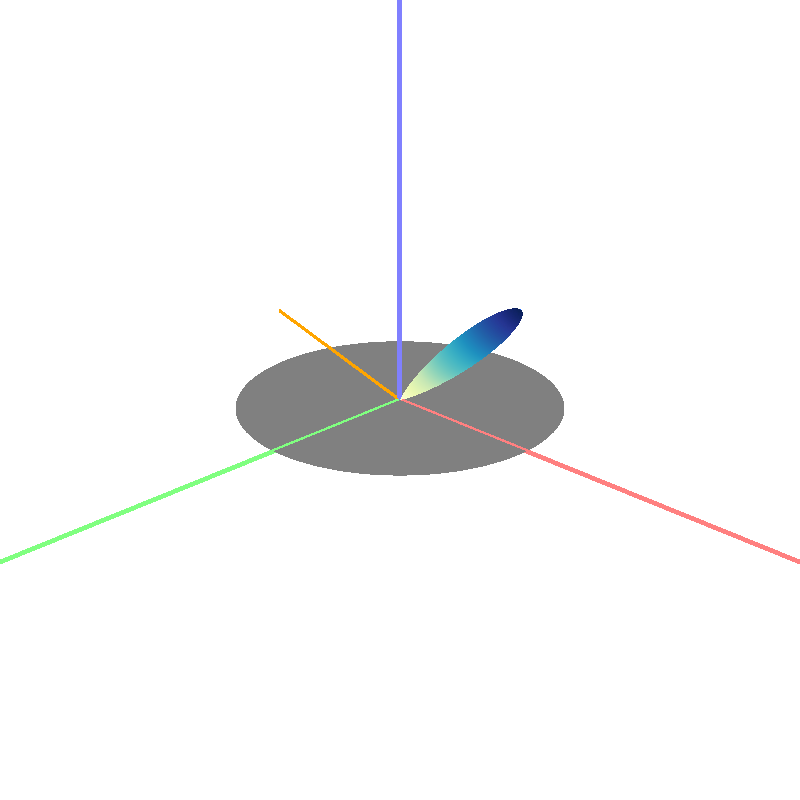
\includegraphics[width=6cm]{Figures/visualizations/brdfPhong.png} }}%
  \qquad
  \subfloat[Vizualizace Blinn-Phong BRDF\label{fig:blinnPhongBRDFRender}]{{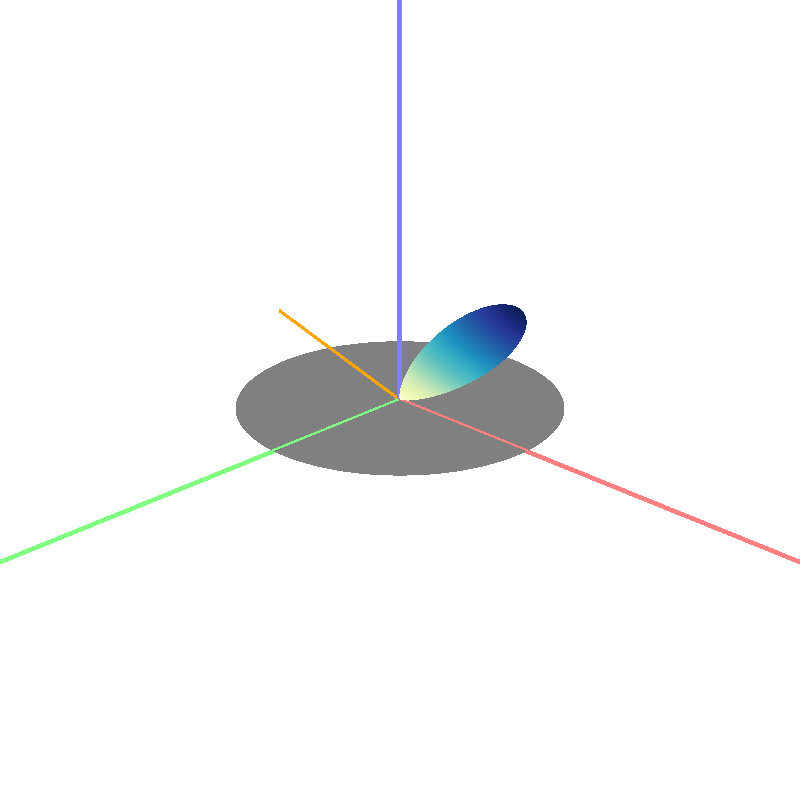
\includegraphics[width=6cm]{Figures/visualizations/brdfBlinnPhong.png} }}%
  \qquad
  \subfloat[Vizualizace fyzikálně korektní verze BRDF podle Phongova modelu\label{fig:physCorrectPhongBRDFRender}]{{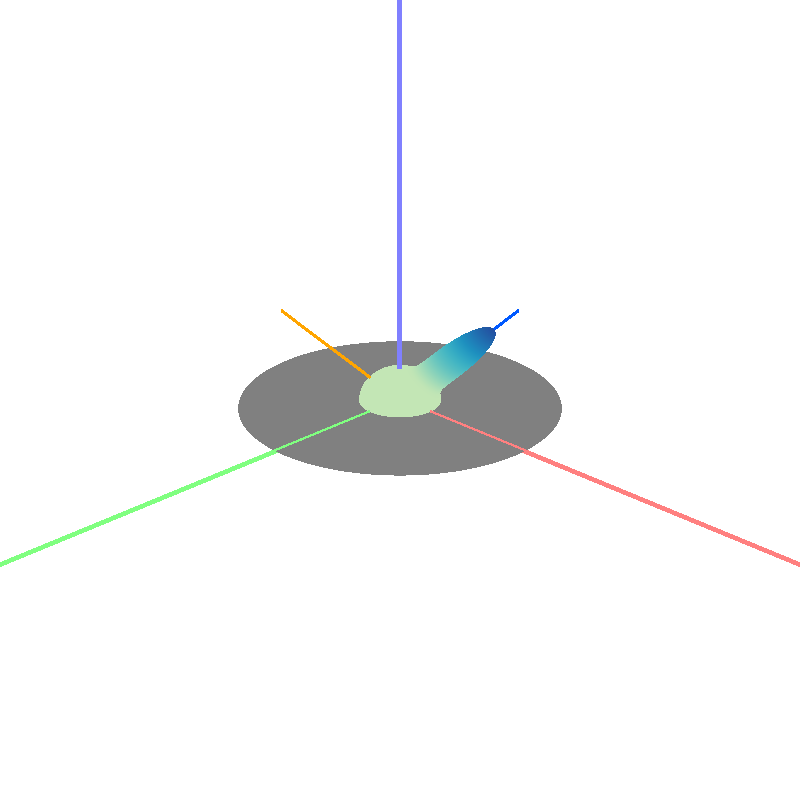
\includegraphics[width=6cm]{Figures/visualizations/brdfPhysCorrectPhong.png} }}%
  \caption{Vizualizace jednotlivých verzí BRDF podle Phongova modelu}%
  \label{fig:allPhongBRDFRender}%
\end{figure}

\subsection{Torrance-Sparrow} \label{sec:torrancesparrow}
Torrance-Sparrow BRDF patří mezi fyzikální modely a je považován za jeden s nejúplnějších modelů~\cite{BRDFOverview}. Mimo jiné je např.\ schopen simulovat odlesk polarizovaného světla. Tento model simuluje mikroploškové materiály a pomocí parametru roughness (drsnost) simuluje mikroskopické nerovnosti materiálu. Orientace mikroskopických nerovností je v materiálu náhodná. Vyšší hodnota drsnosti materiálu snižuje lesklost materiálu. Torrance-Sparrow BRDF funkce je definována \hyperref[eq:TorranceSparrow]{vzorcem~\ref{eq:TorranceSparrow}}. Ukázka vizualizace je zobrazena na \hyperref[fig:torranceSparrowBRDFRender]{obrázku~\ref{fig:torranceSparrowBRDFRender}} s parametry \(\rough=0{,}35,~\Fzero = 1\)\par

\begin{equation}\label{eq:TorranceSparrow}
  \brdf  =  \frac{k_d}{\pi} + \frac{k_s D(\halfVec,\rough) F(\outVec) G(\outVec,\inVec, \normMicroVec)}{4\pi (\normVec \cdot \inVec)}\,.
\end{equation}

Pro výpočet se používá distribuční funkce \(D\), která popisuje rozložení normál mikroplošek. V této konkrétní implementaci je použita Beckmannova distribuční funkce

\begin{equation}\label{eq:beckDistr}
  D(\halfVec,\rough)  =  \frac{e^{\left(\frac{(\normVec\cdot \halfVec)^{2}-1}{\rough^{2}(\normVec \cdot \halfVec)^{2}}\right)}}{\rough^2(\normVec\cdot \halfVec)^{2}}\,.
\end{equation}

Beckmannova distribuční funkce pracuje s normálou mikroplošky (kolem které se generuje rozložení) a hodnotou drsnosti materiálu. Jako normála mikroplošky je použit poloviční vektor mezi pohledovým a světelným vektorem (viz \hyperref[sec:Phong]{\ref{sec:Phong} Phong}) z důvodu, že mikroploška perfektně odráží světlo právě v případě, kdy je normála mikroplošky shodná s polovičním vektorem \(\halfVec\)~\cite{PHARR2017507}.\par
Dále se počítá poměr odraženého světla a lomeného světla \(F\) pomocí Fresnelových vzorců. Pro výpočet je použita Schlickova aproximace \hyperref[eq:schlickFresnel]{\ref{eq:schlickFresnel}}~\cite{SchlickFresnel}

\begin{equation}\label{eq:schlickFresnel}
  F(\outVec)  \approx R(\theta) = \Fzero + {(1-\Fzero)}{(1-\cos\theta)}^{5}\,.
\end{equation}

Poslední část pro výpočet je koeficient geometrického útlumu \(G\), který vyjadřuje zakrytí mikroplošek při odrazu světla \hyperref[eq:geomAtatenuation]{\ref{eq:geomAtatenuation}}~\cite{BRDFOverview}

\begin{equation}\label{eq:geomAtatenuation}
  G(\outVec,\inVec, \normMicroVec)  =  \min \left( 1, \frac{2 ( \normVec \cdot \halfVec ) ( \normVec \cdot \outVec )
    }{ ( \outVec \cdot \halfVec ) },\frac{ 2 ( \normVec \cdot \halfVec ) ( \normVec \cdot \inVec ) }{ ( \outVec \cdot \halfVec ) } \right)\,.
\end{equation}


Ve článku~\cite{MicrofacetWalter} byly uvedeny podmínky pro distribuční funkce \(D\) a funkce pro výpočet geometrického útlumu \(G\), které by měly být splněny, aby byly výsledky realistické. Pro distribuční funkce \(D\) by mělo být splněno:
\begin{itemize}
  \item Hodnota distribuční funkce je nezáporná, \(D(\halfVec,\rough) \in \intervalco{0}{\infty}\).
  \item Celková plocha mikroplošek povrchu tělesa je větší nebo rovna ploše povrchu tělesa.
  \item Zobrazená plocha mikroplošek je stejná jako zobrazená plocha povrchu tělesa.
\end{itemize}
Funkce geometrického útlumu \(G\) by měly splňovat alespoň následující podmínky:
\begin{itemize}
  \item Pro hodnotu funkce geometrického útlumu platí: \(G(\outVec, \inVec, \normMicroVec) \in \intervalcc{0}{1}\).
  \item Funkce útlumu by měla být symetrická, platí \(G(\outVec, \inVec, \normMicroVec) = G(\inVec, \outVec, \normMicroVec)\).
  \item Zadní strana mikroplošky by neměla být viditelná v případě pohledu na přední stranu makroplošky a naopak.
\end{itemize}

\begin{figure}[ht]%
  \centering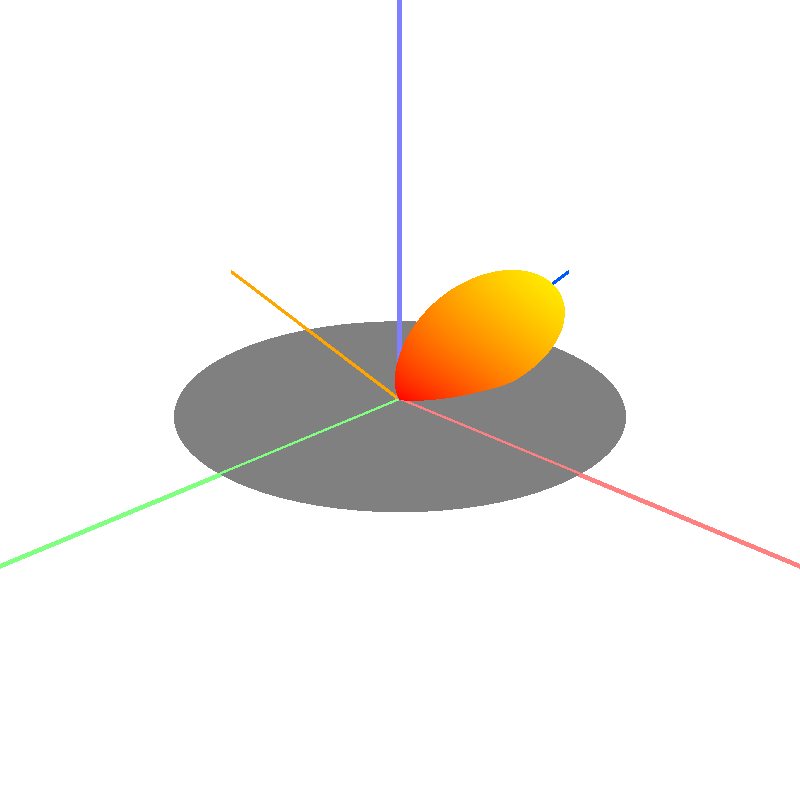
\includegraphics[width=6cm]{Figures/visualizations/brdfTorranceSparrow.png}%
  \caption{Vizualizace Torrance-Sparrow BRDF}%
  \label{fig:torranceSparrowBRDFRender}%
\end{figure}

\subsection{Cook-Torrance}
Cook-Torrance BRDF rozšiřuje mikroploškové BRDF o myšlenku, že pouze mikroplošky orientované podél vektoru \(\halfVec\) mají vliv na výsledný odraz světla. Pro výpočet odrazové složky jsou využity opět funkce \(F, D, G\) (viz \hyperref[sec:torrancesparrow]{\ref{sec:torrancesparrow} Torrance-Sparrow}). Cook-Torrance BRDF se vypočítá \hyperref[eq:CookTorrance]{vzorcem~\ref{eq:CookTorrance}}~\cite{CookTorranceBRDF}

\begin{equation} \label{eq:CookTorrance}
  \brdf  = \frac{F(\outVec) D(\halfVec,\rough) G(\outVec,\inVec)}{4 (\normVec\cdot\inVec) (\normVec\cdot\outVec)}\,.
\end{equation}

Nevýhodou této BRDF funkce je nesplnění fyzikální přesnosti z důvodu nesplnění zákona zachování energie pro některé \(\left(\outVec,\inVec\right)\)~\cite{BRDFOverview}. Ukázka vizualizace je zobrazena na \hyperref[fig:cookTorranceBRDFRender]{obrázku~\ref{fig:cookTorranceBRDFRender}} s parametry \(\rough=0{,}7,~\Fzero = 0{,}6\).


\begin{figure}[ht]%
  \centering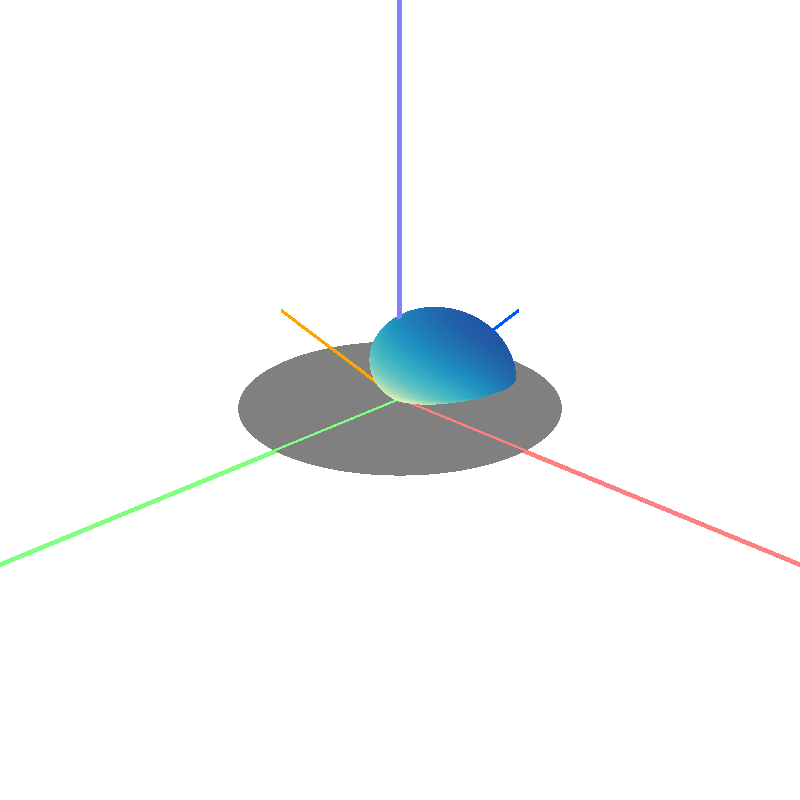
\includegraphics[width=6cm]{Figures/visualizations/brdfCookTorrance.png}%
  \caption{Vizualizace Cook-Torrance BRDF}%
  \label{fig:cookTorranceBRDFRender}%
\end{figure}

\subsection{Oren-Nayar}
Oren-Nayar BRDF popisuje Lambertovské difusivní materiály. Na rozdíl od BRDF podle Beer-Lambertova zákona (\hyperref[sec:Lambert]{viz~\ref{sec:Lambert} Lambert}) pracuje Oren-Nayar BRDF s mikroploškami, které si lze představit jako mikroskopické nerovnosti ve tvaru písmena \textquote{V}. Dále, na rozdíl od jiných mikroploškových modelů (\hyperref[sec:torrancesparrow]{Torrance-Sparrow}) nejsou mikroplošky odrazivé, ale difuzivní. Oren-Nayar BRDF bere v úvahu odrazy světla mezi jednotlivými mikroploškami s limitovaným maximálním počtem odrazů mezi dvojicí mikroplošek. Pro generování distribuce orientace mikroplošek je použito Gaussovo rozdělení, které je nastavena pomocí parametru \(\rough\). Parametr \(\rough\) určuje směrodatnou odchylku úhlu orientace mikroplošky.~\cite{BRDFOverview, OrenNayar}. Oren-Nayar BRDF je definováno \hyperref[eq:OrenNayar]{vzorcem~\ref{eq:OrenNayar}}

\newcommand{\cosphiri}{\cos\left(\phi_r-\phi_i\right)}

\begin{eqnarray}
  \alpha & = & \max(\theta_i , \theta_o) = \max(\arccos(\normVec\cdot\inVec), \arccos(\normVec\cdot\outVec)) \nonumber \\
  \beta & = & \min(\theta_i , \theta_o) = \min(\arccos(\normVec\cdot\inVec), \arccos(\normVec\cdot\outVec)) \nonumber \\
  \cosphiri & = & \widehat{\left( \inVec - \normVec(\normVec\cdot\inVec) \right)} \cdot \widehat{\left( \outVec - \normVec(\normVec\cdot\outVec)  \right)} \nonumber \\
  C_1 & = & 1-0{,}5\frac{\rough^{2}}{\rough^{2} + 0{,}33} \nonumber \\
  C_2 & = & \left\{\begin{matrix*}[l] 0{,}45\frac{\rough^{2}}{\rough^{2}+0{,}09}\sin\alpha & \cosphiri \geq 0\\ 0{,}45\frac{\rough^{2}}{\rough^2+0{,}09}\left(\sin\alpha-\left(\frac{2\beta}{\pi}\right)^{3}\right) & jinak \end{matrix*}\right. \nonumber \\
  C_3 & = & 0{,}125\left(\frac{\rough^2}{\rough^2 + 0{,}009}\right)\left(\frac{4\alpha\beta}{\pi^2}\right)^{2} \nonumber \\
  L^{1}_{r} & = & \frac{\alb}{\pi}\left[C_1 + \cosphiri C_2\tan\beta + \left( 1-\left | \cosphiri  \right | \right)C_3\tan \left(\frac{\alpha+\beta}{2}\right)\right] \nonumber \\
  L^{2}_{r} & = & 0{,}17\frac{\alb^{2}}{\pi}\frac{\rough^{2}}{\rough^2+0{,}13}\left[1 - \cosphiri  \left(\frac{2\beta}{\pi}\right)^{2} \right] \nonumber \\
  \brdf & = & L^{1}_{r} + L^{2}_{r}\,. \label{eq:OrenNayar}
\end{eqnarray}

Ukázka vizualizace je zobrazena na \hyperref[fig:orenNayarBRDFRender]{obrázku~\ref{fig:orenNayarBRDFRender}} s parametry \(\rough=0{,}7,~\alb = 0{,}8\).

\begin{figure}[ht]%
  \centering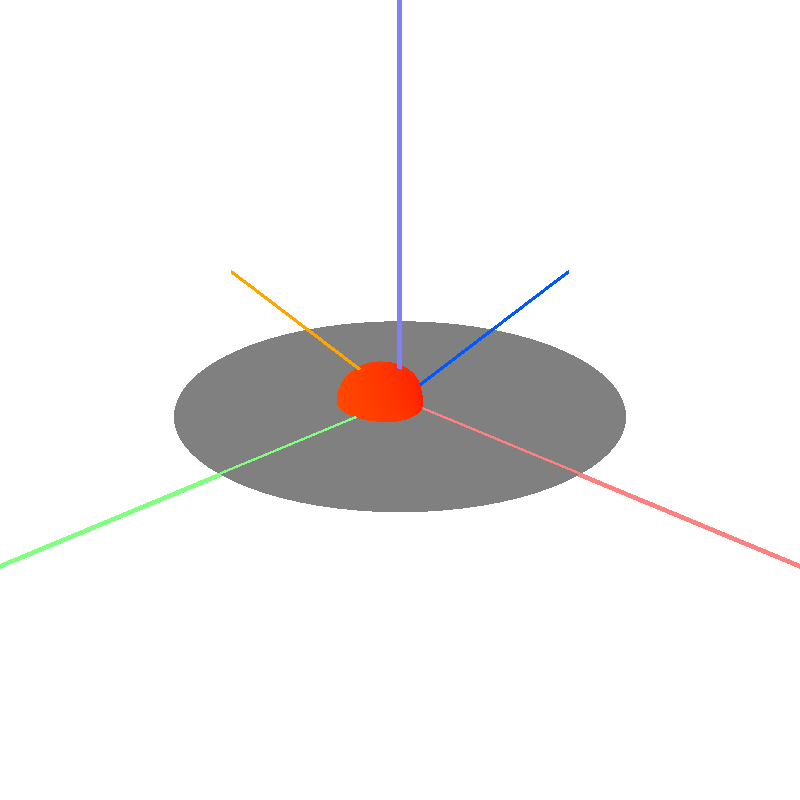
\includegraphics[width=6cm]{Figures/visualizations/brdfOrenNayar.png}%
  \caption{Vizualizace Oren-Nayar BRDF}%
  \label{fig:orenNayarBRDFRender}%
\end{figure}

\section{Srovnání náročnosti výpočtu BRDF funkcí}
Následující kapitoly se zabývají srovnáním jednotlivých BRDF funkcí dle jejich výpočetní složitosti.
\subsection{Metodika výpočtu výpočetní složitosti}
Při výpočtu složitosti jsem se rozhodl pro praktické měření výkonu jednotlivých algoritmů, protože výsledná hodnota má pro praktickou implementaci vyšší informační hodnotu než teoretická analýza. Jako metriku jsem zvolil absolutní a relativní čas výpočtu řádově \(10^7\) iterací výpočtu. Výsledky měření jsem pak rozdělil do tří kategorií - celkové srovnání, srovnání BRDF funkcí pro difuzní povrchy a srovnání BRDF funkcí pro lesklé povrchy.

\subsection{Výsledky měření, zhodnocení}
Konkrétní výsledky měření jsou uvedeny v tabulkách \hyperref[tab:DiffuseBRDFsComparison]{\ref{tab:DiffuseBRDFsComparison}}, \hyperref[tab:GlossyBRDFsComparison]{\ref{tab:GlossyBRDFsComparison}} a \hyperref[tab:AllBRDFsComparison]{\ref{tab:AllBRDFsComparison}}.  Z výsledků z \hyperref[tab:DiffuseBRDFsComparison]{tabulky~\ref{tab:DiffuseBRDFsComparison}} vyplývá, že BRDF podle Beer-Lambertova zákona je z hlediska výpočetního výkonu nejefektivnější BRDF funkce pro matné povrchy. Tento výsledek je očekávatelný z důvodu velmi jednoduchého vzorce. Oproti BRDF podle Beer-Lambertova zákona ale Oren-Nayar poskytuje širší možnosti nastavení díky parametru drsnosti. Oren-Nayar tak může věrněji reprezentovat drsnější difuzivní materiály.\par
Ze srovnání BRDF funkcí pro lesklé povrchy v \hyperref[tab:GlossyBRDFsComparison]{tabulce~\ref{tab:GlossyBRDFsComparison}} vyplývá, že mezi jednotlivými složitějšími funkcemi není rozdíl příliš markantní. BRDF funkce dokonalého odrazu je opět dle očekávání nejefektivnější. Pozornost si zaslouží rozdíl mezi tradičním BRDF podle Phongova modelu a jeho fyzikálně přesnou variantou. Je vidět, že přidáním fyzikální korektnosti se výkon zhoršil pouze o cca \(16~\%\).

\begin{table}[ht]
  \centering
  \begin{tabular}{ld{3}d{3}}
    \toprule
    BRDF Funkce & \multicolumn{1}{r}{Absolutní čas} & \multicolumn{1}{r}{Relativní čas} \\
    \midrule
    Lambert     & 0.05~\text{s}                     & 1.00                              \\
    Oren-Nayar  & 1.36~\text{s}                     & 28.36                             \\
    \bottomrule
  \end{tabular}
  \caption{Srovnání BRDF funkcí pro matné povrchy}
  \label{tab:DiffuseBRDFsComparison}
\end{table}

\begin{table}[ht]
  \centering
  \begin{tabular}{ld{3}d{3}}
    \toprule
    BRDF Funkce              & \multicolumn{1}{r}{Absolutní čas} & \multicolumn{1}{r}{Relativní čas} \\
    \midrule
    Mirror                   & 0.04~\text{s}                     & 1.00                              \\
    Phong                    & 0.41~\text{s}                     & 10.84                             \\
    Physically correct Phong & 0.48~\text{s}                     & 12.79                             \\
    Blinn-Phong              & 0.50~\text{s}                     & 13.25                             \\
    Cook-Torrance            & 0.53~\text{s}                     & 13.98                             \\
    Torrance-Sparrow         & 0.54~\text{s}                     & 14.18                             \\
    \bottomrule
  \end{tabular}
  \caption{Srovnání BRDF funkcí pro lesklé povrchy}
  \label{tab:GlossyBRDFsComparison}
\end{table}

\clearpage
\chapter{Vizualizační aplikace}
Aplikace jako taková umožňuje zobrazit BRDF funkce popsané v kapitole \hyperref[sec:brdffunctions]{\ref{sec:brdffunctions} Přehled BRDF funkcí}. Důležitým prvkem je také interaktivita, kdy je možné měnit jednotlivé parametry BRDF funkcí. Kromě samotných BRDF funkcí aplikace umožňuje zobrazit i metody pro vzorkování funkcí (toto téma je dále rozebráno v kapitole \hyperref[sec:reduction]{\ref{sec:reduction} Redukce variance Monte Carlo}), kdy je možné přepínat mezi jednotlivými BRDF funkcemi a vzorkovacími funkcemi. Je tedy možné demonstrovat důležitost správného výběru vzorkovací funkce k vybrané BRDF funkci. Pro doplnění funkcionality obsahuje aplikace také možnost pro uložení snímku aktuální vizualizace BRDF ve vysokém rozlišení.\par
Poslední funkcionalitou je interaktivní okno s jednoduchou scénou, která je renderována s použitím aktuálně vybrané BRDF funkce. Pro jednoduchost je renderován model koule, který je popsán analyticky. Tato testovací scéna je primárně osvětlena HDR obrazem, ale aplikace také umožňuje osvětlit scénu konstantním jasem. Tímto nastavením je simulována situace, kdy na objekt dopadá ze všech směrů stejné množství světla. Takto osvětlená scéna je známa jako tzv.\ furnace test a slouží pro kontrolu fyzikální korektnosti BRDF funkce. Ukázka uživatelského rozhraní aplikace je zobrazena na \hyperref[fig:myapp]{obrázku~\ref{fig:myapp}}.\par
Následující odstavce se zabývají konkrétními detaily implementace a popisem technických řešení použitých pro jednotlivé funkce implementované vizualizační aplikace.

\begin{figure}[ht]
  \centering
  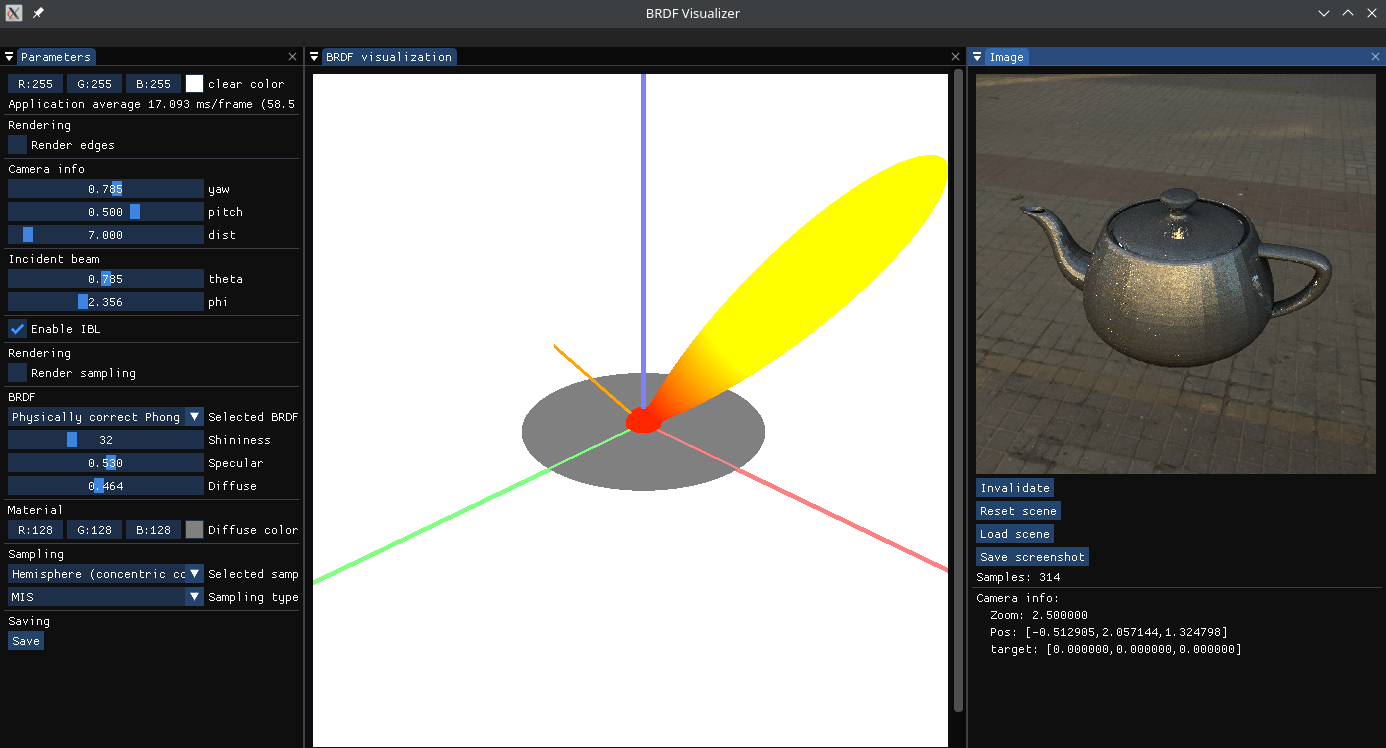
\includegraphics[width=15cm]{Figures/visualizations/MyBRDFVizApp.png}
  \caption{Uživatelské rozhraní vytvořené aplikace}%
  \label{fig:myapp}%
\end{figure}

\section{Vizualizace BRDF}
Při implementaci jsem se chtěl co nejvíce přiblížit standardním referenčním obrázkům popisujícím princip BRDF funkcí (viz \hyperref[fig:brdf2D]{obrázek~\ref{fig:brdf2D}}). Výsledná vizualizace znázorňuje  pro daný vstupní směr všechny možné výstupní směry, do kterých se světlo odráží. Této vizualizace se dá jednoduše dosáhnout tak, že se vygeneruje jednotková hemisféra a jednotlivé body na hemisféře jsou posunuty o hodnotu BRDF funkce pro daný vstupní a výstupní směr. Každý bod na hemisféře zvýrazňuje výstupní směr, vzdálenost bodu od středu (délka vektoru) zvýrazňuje hodnotu BRDF funkce.\par
Pro vizualizaci jsem se rozhodl vygenerovat jednotkovou polokouli a jednotlivé body polokoule upravit v OpenGL Vertex shaderu. Při generování polokoule jsem narazil na problém, kdy pro vizualizaci bylo potřeba mít co nejrovnoměrněji rozložené polygony, ideálně všechny s podobnou velikostí. Rozhodl jsem se tedy negenerovat UV kouli, ale geodetický mnohostěn (srovnání na \hyperref[fig:spheresComparison]{obrázku~\ref{fig:spheresComparison}}), který je tvořen rovnostrannými trojúhelníky.\par

\begin{figure}[ht]
  \centering
  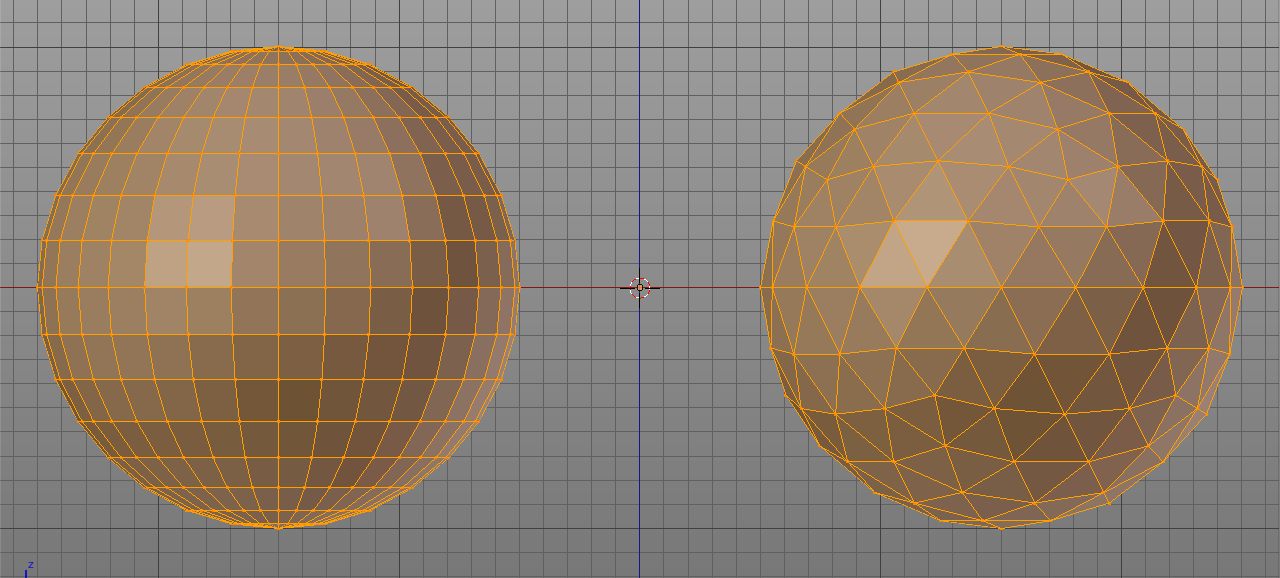
\includegraphics[width=10cm]{Figures/IcosphereUVSphereComparison.png}
  \caption[Srovnání UV koule a geodetického mnohostěnu]{Srovnání UV koule a geodetického mnohostěnu~\cite{tan_2019}}
  \label{fig:spheresComparison}
\end{figure}

Pro zjednodušení implementace jsem vycházel z kódu pro dvacetistěn~\cite{OpenGLSphere}, jehož trojúhelníkové stěny jsem dále rekurzivně dělil. Počet rekurzivních dělení určuje rozlišení výsledné vizualizace, s vyšším počtem dělení se zvyšuje rozlišení.
Generování hemisféry probíhá v následujících krocích:
\begin{enumerate}
  \item Vygenerování dvacetistěnu (viz \hyperref[fig:icasehedron]{obrázek~\ref{fig:icasehedron}})
  \item Rozdělení dvacetistěnu na poloviční dvacetistěn (viz \hyperref[fig:halficasehedron]{obrázek~\ref{fig:halficasehedron}})
  \item Rekurzivní dělení polygonů až do dosažení požadované jemnosti povrchu (viz \hyperref[fig:halficasehedron1]{obrázek 1\(\times\) rozdělených polygonů~\ref{fig:halficasehedron1}} a \hyperref[fig:halficasehedron3]{obrázek  3\(\times\) rozdělených polygonů~\ref{fig:halficasehedron3}})
\end{enumerate}
Postup generování hemisféry použité pro vykreslení BRDF funkcí je zobrazen na \hyperref[fig:hemisfera]{obrázku~\ref{fig:hemisfera}}.\par

\begin{figure}[ht]%
  \centering
  \subfloat[\label{fig:icasehedron}]{{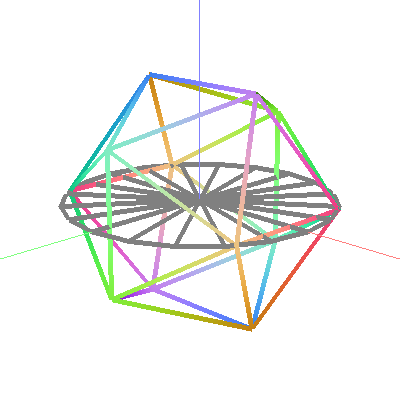
\includegraphics[width=6cm]{Figures/icosphere.png} }}%
  \qquad
  \subfloat[\label{fig:halficasehedron}]{{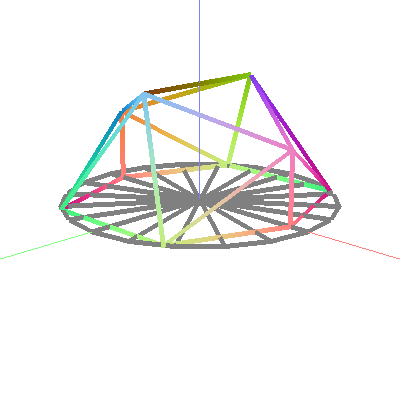
\includegraphics[width=6cm]{Figures/halficosphere.png} }}%
  \qquad
  \subfloat[\label{fig:halficasehedron1}]{{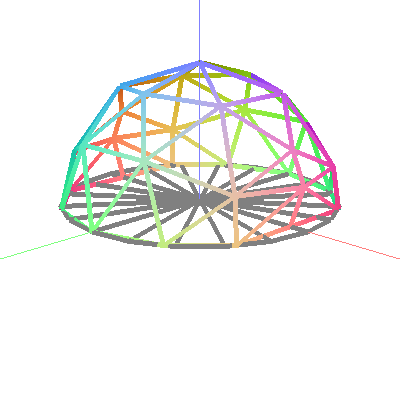
\includegraphics[width=6cm]{Figures/halficosphere1.png} }}%
  \qquad
  \subfloat[\label{fig:halficasehedron3}]{{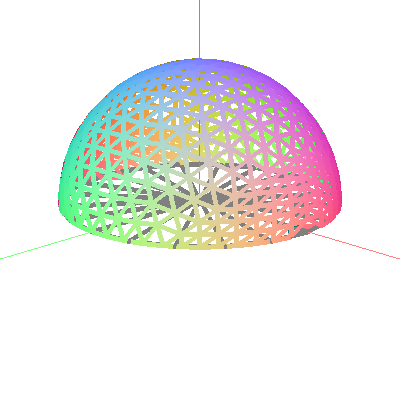
\includegraphics[width=6cm]{Figures/halficosphere3.png} }}%
  \caption{Postup generování hemisféry}%
  \label{fig:hemisfera}%
\end{figure}

Body takto generované hemisféry jsou následně upraveny ve vertex shaderu. Základní kód pro úpravu hemisféry glsl vertex shaderem je uveden ve \hyperref[src:vertexbrdf]{výpise~\ref{src:vertexbrdf}}. Vertex shader pracuje se vstupními parametry \texttt{in\_Position}, \texttt{u\_incidentVector} a parametry pro jednotlivé BRDF funkce. Pro jednoduchost je výpis zkrácen a zjednodušen. Parametr \texttt{in\_Position} určuje vstupní bod hemisféry a před vstupem do BRDF funkce je normalizován (aby byla pojištěna jednotková vzdálenost od středu). Parametr \texttt{u\_incidentVector} představuje směrový vektor \(\outVec\).\par

\begin{listing}[ht]
  \inputminted{c++}{sampleshader.glsl}
  \caption{Zjednodušený vertex shader}
  \label{src:vertexbrdf}
\end{listing}

Ve vertex shaderu jsou poté ve funkci \texttt{BRDF} implementovány jednotlivé BRDF funkce. Pro přepínání mezi aktuálně zvolenou BRDF funkcí slouží uniformní proměnná, která je do shaderu předávána z programu. Parametry jednotlivých funkcí jsou také předávány pomocí uniformních proměnných. Po zpracování ve vertex shaderu je následně vizualizace zpracována fragment shaderem, kde je každý bod vizualizace jednoduše obarven podle vzdálenosti bodu od středu (tzn.\ dle hodnoty BRDF funkce daného bodu). Obarvení dané hodnoty BRDF funkce je provedeno za pomocí sekvenční barevné mapy \textquote{Autumn} (viz \hyperref[fig:colormap]{obrázek~\ref{fig:colormap}}). Ukázka výsledné vizualizace je zobrazena na \hyperref[fig:myapp]{obrázku uživatelského rozhraní aplikace~\ref{fig:myapp}} v hlavním okně, kde je vizualizována fyzikálně korektní verze BRDF podle Phongova modelu.

\begin{figure}[ht]
  \centering
  
\includegraphics[width=8cm]{Figures/MATLAB_autumn.png}
  \caption{Barevná škála použitá pro obarvení BRDF funkcí}%
  \label{fig:colormap}%
\end{figure}

\clearpage
\section{Vizualizace vzorkování} \label{sec:samplingViz}
Každou BRDF funkci je vhodné kombinovat s vhodně zvolenou vzorkovací funkcí. Výběr vzorkovací funkce je důležitý z důvodu optimálního generování vektorů. Na \hyperref[fig:samplingExample]{obrázku~\ref{fig:samplingExample}} jsou zobrazeny dvojice dvou BRDF funkcí a vzorkovacích funkcí. Z obrázku je vidět, že např.\ vzorkovací funkce \hyperref[fig:samplingExampleLambert]{obrázku~\ref{fig:samplingExampleLambert}} není optimální pro  BRDF funkci na \hyperref[fig:samplingExamplePhongBRDF]{obrázku~\ref{fig:samplingExamplePhongBRDF}}. Velké množství vektorů je vygenerováno mimo lalok této BRDF funkce. Opačným extrémem by bylo zvolení kombinace vzorkovací funkce na \hyperref[fig:samplingExamplePhong]{obrázku~\ref{fig:samplingExamplePhong}} a BRDF funkce na \hyperref[fig:samplingExampleLambertBRDF]{obrázku~\ref{fig:samplingExampleLambertBRDF}}. V takovém případě vzorkovací funkce nepokryje celou BRDF funkci. Detaily jednotlivých implementovaných vzorkovacích funkcí jsou podrobněji popsány v kapitole \hyperref[sec:reduction]{\ref{sec:reduction} Redukce variance Monte Carlo}.\par
K vizualizaci vzorkovacích funkcí jsem se rozhodl přistoupit pomocí vizualizace vektory. Princip je v zásadě jednoduchý. Vzorkovací funkce pracují tak, že se vygeneruje směr pro náhodně vygenerované hodnoty \(\randU\) a \(\randV\). Vizualizace potom funguje na principu vygenerování uniformně rozložených hodnot v mřížce s daným rozlišením. Takto generované hodnoty jsou poté převedeny pomocí vzorkovací funkce do vektorů. Uniformně rozložené generované vektory jsou poté přímo zobrazeny, barva každého vektoru přímo koresponduje s jeho směrem. V případě potřeby je možné interaktivně zvýšit nebo snížit počet vizualizovaných vzorků. Ve výchozím nastavení je délka jednotlivých vizualizovaných vektorů jednotková. Je také možné nastavit násobení velikostí vektorů hodnotou pdf. Násobení velikosti vektoru hodnotou pdf demonstruje rozložení pravděpodobnosti vzorku. Čím větší je velikost vzorku, tím větší je jeho pravděpodobnost. Na \hyperref[fig:samplingExamplePhong]{obrázcích~\ref{fig:samplingExamplePhong}} a \hyperref[fig:samplingExampleLambert]{\ref{fig:samplingExampleLambert}} jsou zobrazeny ukázky vizualizací vzorkovacích funkcí.

\begin{figure}[ht]%
  \centering
  \subfloat[\label{fig:samplingExamplePhongBRDF}]{{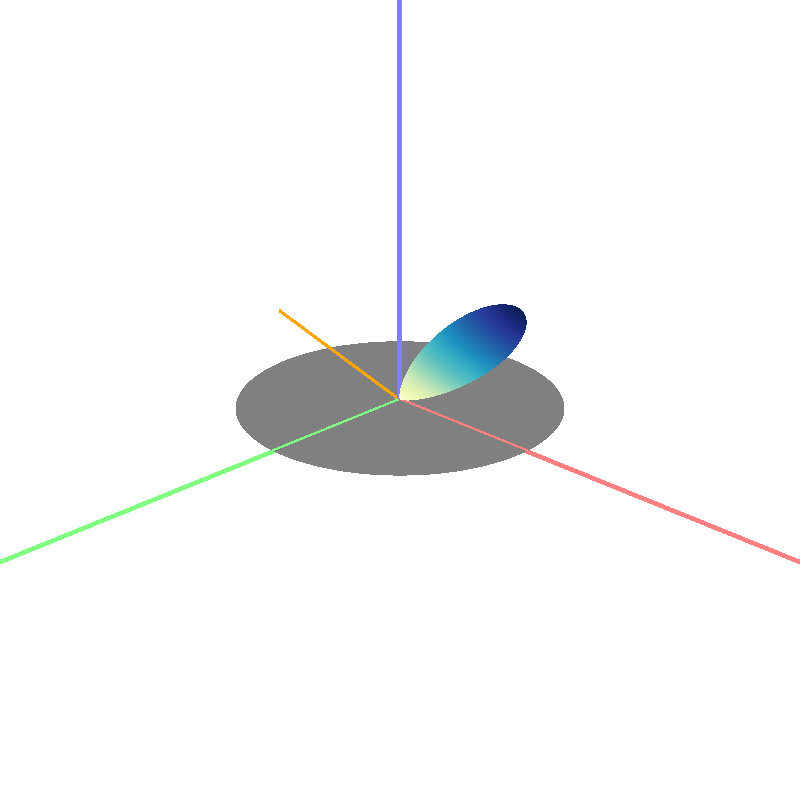
\includegraphics[width=6cm]{Figures/visualizations/brdfBlinnPhong.png} }}%
  \qquad
  \subfloat[\label{fig:samplingExamplePhong}]{{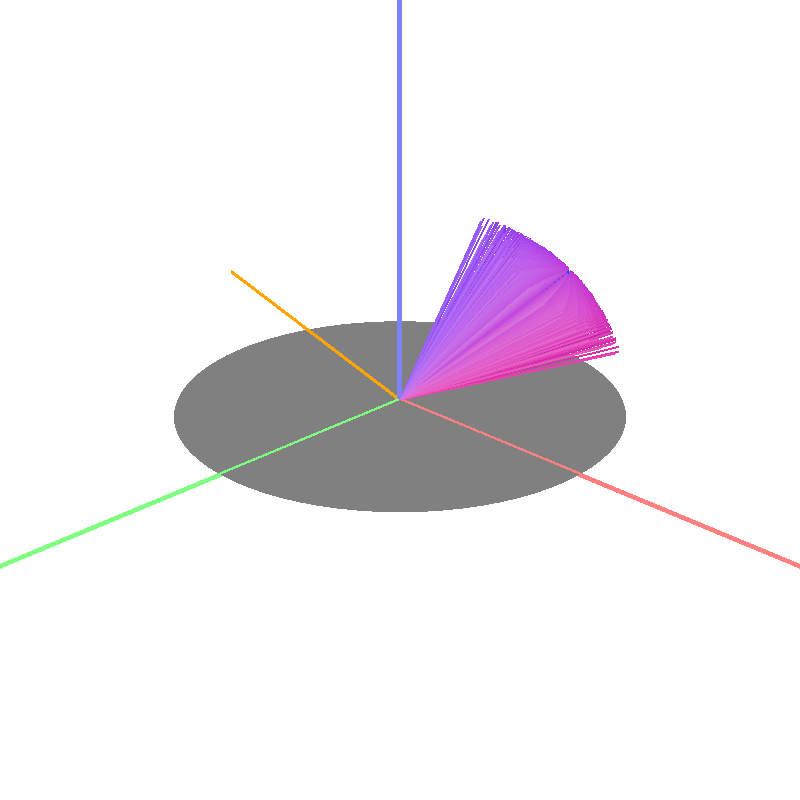
\includegraphics[width=6cm]{Figures/visualizations/samplingSpecular.png} }}%
  \qquad
  \subfloat[\label{fig:samplingExampleLambertBRDF}]{{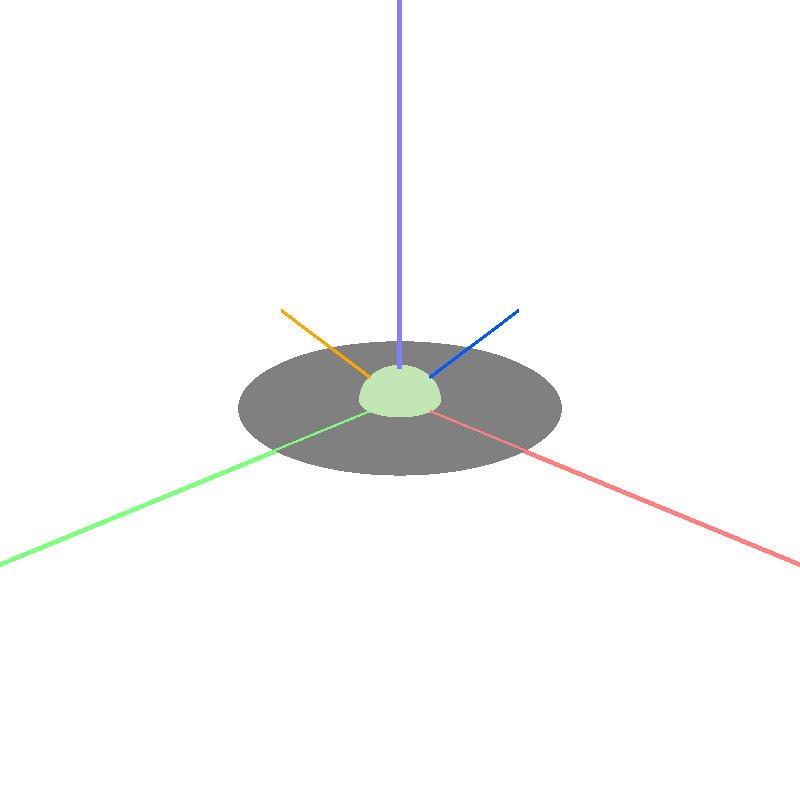
\includegraphics[width=6cm]{Figures/visualizations/brdfLambert.png} }}%
  \qquad
  \subfloat[\label{fig:samplingExampleLambert}]{{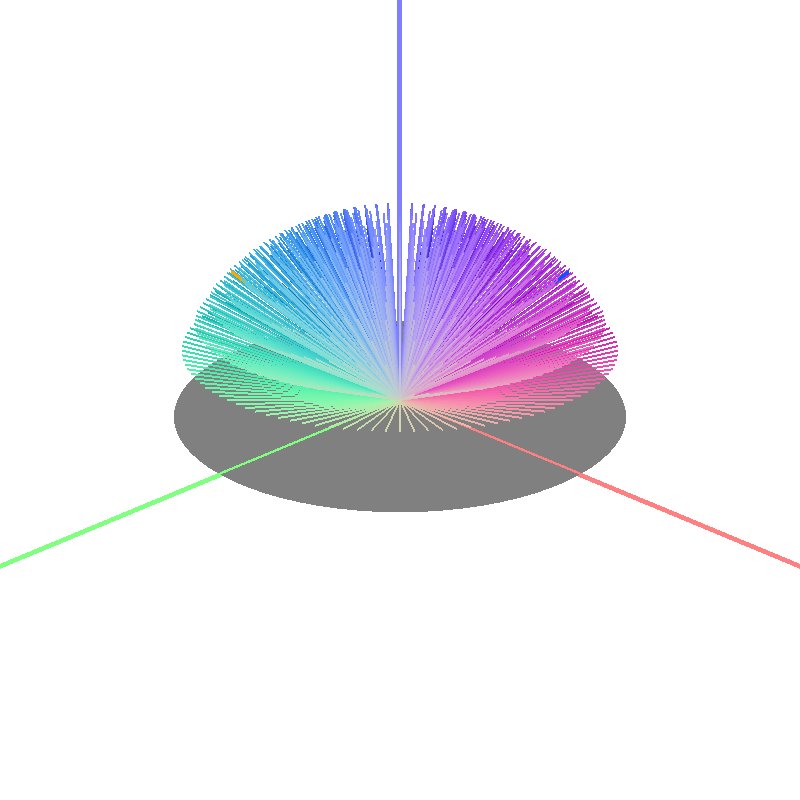
\includegraphics[width=6cm]{Figures/visualizations/samplingCosWeight.png} }}%
  \caption{BRDF funkce a korespondující vzorkovací funkce }%
  \label{fig:samplingExample}%
\end{figure}

\section{Vizualizace výsledku path tracingu}
Pro ukázku výsledku je vizualizován také výsledný render. Jak již bylo zmíněno, vizualizována je koule, která je osvětlena HDR mapou, nebo konstantním pozadím.\par
Pro výpočet osvětlení je využita metoda Monte Carlo, v path traceru jsou také implementovány funkce pro optimalizaci výpočtu. Pro ukázku volby vzorkovací funkce využívá path tracer vzorkovací funkci zvolenou v ovládacím panelu. Jednotlivé vzorkovací funkce jsou podrobněji popsány v kapitole \hyperref[sec:reduction]{\ref{sec:reduction} Redukce variance Monte Carlo}. Implementováno je také vzorkování světelných zdrojů z HDR mapy. Vzorkování světelných zdrojů je možné v ovládacím panelu zapínat a vypínat pro demonstraci efektů jednotlivých typů vzorkování na výsledném renderu.\par
Kromě analyticky zadané koule je také možné vizualizovat render libovolného načteného objektu. Pro urychlení výpočtu je načtený objekt uložen do BVH stromu -- akcelerační struktury, dále popsané v kapitole \hyperref[sec:reduction]{\ref{sec:reduction} Redukce variance Monte Carlo}. Výsledný render modelu je zobrazen na obrázcích \hyperref[fig:loadedObjectRender]{\ref{fig:loadedObjectRender}} a \hyperref[fig:analSphereObjectRender]{\ref{fig:analSphereObjectRender}}.

\begin{listing}[ht]
  \inputminted{python}{pathTracer.py}
  \caption{Pseudokód pro path tracer}
  \label{src:pathtracer}
\end{listing}

\begin{figure}[ht]%
  \centering
  \subfloat[Render načteného objektu \label{fig:loadedObjectRender}]{{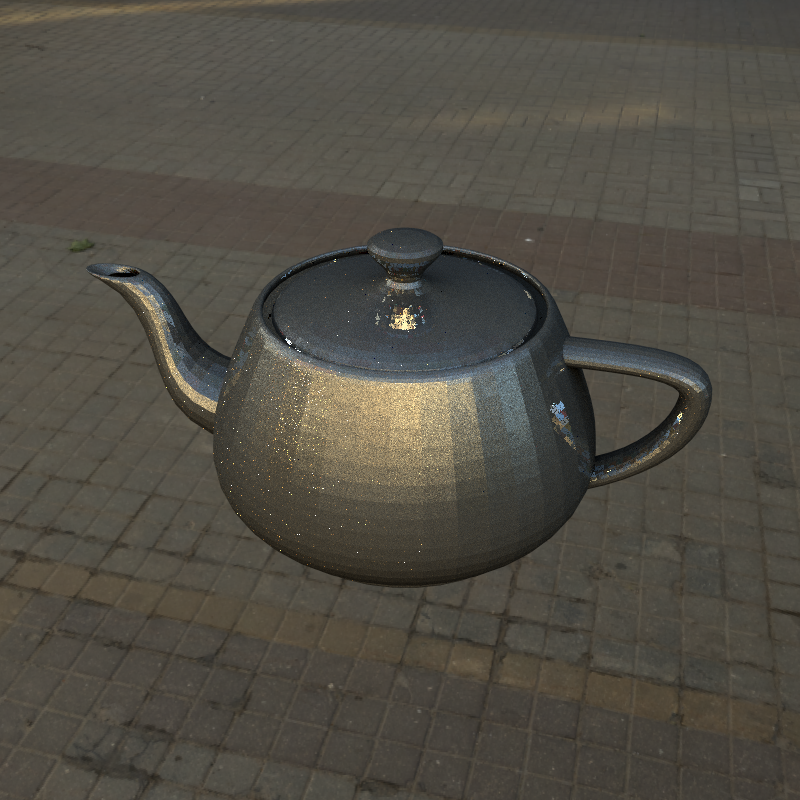
\includegraphics[width=6cm]{Figures/visualizations/teapot.png} }}%
  \qquad
  \subfloat[Render analyticky zadané koule \label{fig:analSphereObjectRender}]{{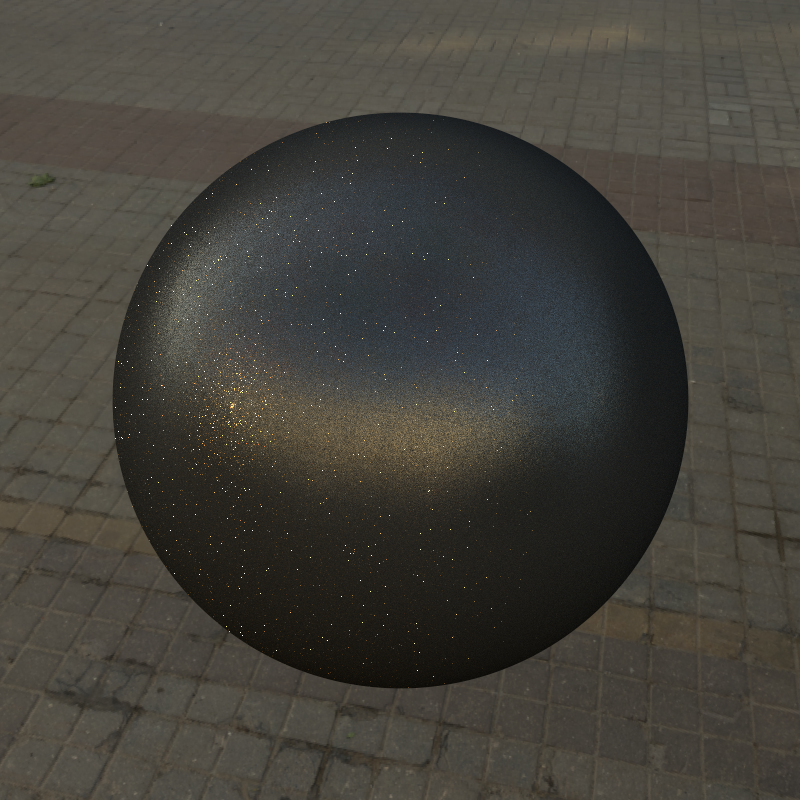
\includegraphics[width=6cm]{Figures/visualizations/sphere.png} }}%
  \caption{Ukázka vizualizace výsledku path tracingu}%
  \label{fig:finalrender}%
\end{figure}

\clearpage
\section{Detaily implementace, použité knihovny a technologie}
Aplikace pro vizualizaci je napsána v moderním C++, s použitím standardu C++17. Při implementaci jsem se snažil v maximální možné míře využívat novou funkcionalitu tohoto standardu.\par
Co se týče architektury mého řešení, je aplikace rozdělena do tří samostatných celků. Hlavní částí aplikace je samotné uživatelské rozhraní, ve kterém jsou všechny ovládací panely. Přímé vykreslování do panelů definovaných knihovnou ImGui není možné, vykreslování jsem tedy prováděl do frame bufferu, resp.\ do textury. Samotné textury jsem poté zobrazoval v ImGui panelech. OpenGL část aplikace se zabývá samotným vykreslováním BRDF funkcí a vzorkování. Embree část aplikace je zodpovědná za vykreslování objektu za pomocí zvolené BRDF funkce.\par
Tato kapitola se nejprve věnuje popisu pomocných matematických funkcí, které jsou použity na různých místech aplikace při práci s vektory. Následně se kapitola věnuje popisu knihoven použitých při implementaci aplikace.

\subsection{Převod vektoru z lokálního do globálního prostoru}
V kapitole \hyperref[sec:reduction]{\ref{sec:reduction} Redukce variance Monte Carlo} jsou popsány metody generování vzorků vektorů používaných pro výpočet odrazu světla. Problémem ale je, že tyto generované vektory nejsou orientovány podél normály. Generované vektory jsou typicky orientovány podle \(\uvec{up}\) vektoru (vektor určující ve scéně osu směrem nahoru). Pro použití vzorku na povrchu s libovolnou normálou je tedy nutné provést rotaci vygenerovaného vektoru podél normálového vektoru. Tato funkce má také využití např.\ při generování vzorků pro odrazovou složku BRDF podle Phongova modelu (viz \hyperref[sec:phongSampling]{\ref{sec:phongSampling} Vzorkování BRDF podle Phongova modelu}). Vzhledem k tomu, že vzorkovací funkce samotná je při renderingu volána velmi často, je vhodné mít všechny kroky vzorkování co nejlépe optimalizované. Jednou z nejlepších metod pro rotaci vektoru je použití transformační matice. Pro rotaci ve 3D prostoru se využívá trojice elementárních rotačních matic, definovaných \hyperref[eq:rotX]{vzorci~\ref{eq:rotX},~\ref{eq:rotY} a~\ref{eq:rotZ}}~\cite{HughesDamEtAl13}\par
\begin{eqnarray}
  R_x(\theta) & = & \begin{pmatrix}
    1 & 0          & 0           \\
    0 & \cos\theta & -\sin\theta \\
    0 & \sin\theta & \cos\theta
  \end{pmatrix} \label{eq:rotX} \\
  R_y(\theta) & = & \begin{pmatrix}
    \cos\theta  & 0 & \sin\theta \\
    0           & 1 & 0          \\
    -\sin\theta & 0 & \cos\theta
  \end{pmatrix} \label{eq:rotY} \\
  R_z(\theta) & = & \begin{pmatrix}
    \cos\theta & -\sin\theta & 0 \\
    \sin\theta & \cos\theta  & 0 \\
    0          & 0           & 1
  \end{pmatrix}\label{eq:rotZ}
\end{eqnarray}
Cílem je získání rotační matice pro rotaci vektoru \(\fromVect\) na vektor \(\toVect\). Po aplikaci rotační matice na vygenerované vektory vzorkovacími funkcemi je dosaženo správné orientace vzorkovaných vektorů. Výpočet rotační matice před dalšími úpravami je definován \hyperref[eq:vectRotation]{vzorcem~\ref{eq:vectRotation}}~\cite{MollerHughesVectRotation}.
\begin{equation} \label{eq:vectRotation}
  \begin{pmatrix}
    u_x^2 + \left ( 1 - u_x^2\right ) \cos\theta                & u_x u_y \left ( 1 - \cos \theta \right ) - y_z \sin \theta & u_x u_z + u_y \sin \theta                                  \\
    u_x u_y \left ( 1 -  \cos \theta \right ) + u_z \sin \theta & u_y^2 + \left ( 1 - u_y^2\right ) \cos\theta               & u_y u_z \left ( 1 - \cos \theta \right ) - u_x \sin \theta \\
    u_x u_z \left ( 1 - \cos \theta \right ) - u_y \sin \theta  & u_y u_z \left ( 1 - \cos \theta \right ) + u_x \sin \theta & u_z^2 + \left ( 1 - u_z^2\right ) \cos\theta
  \end{pmatrix}
\end{equation}
Pro výpočet se používá parametr \(u\), což je normalizovaný vektor kolmý na vektory \(\fromVect\) a \(\toVect\). Z rovnice je také možné odstranit výpočet goniometrických funkcí, vzhledem k tomu, že platí: \(\cos \theta = \fromVect \cdot \toVect\) a \(\sin \theta = \left\Vert \fromVect \times \toVect \right\Vert\). Pro zjednodušení značení je možné provést substituce \hyperref[eq:subst]{\ref{eq:subst}}.

\begin{eqnarray} \label{eq:subst}
  c &=& \fromVect \cdot \toVect \nonumber\\
  v &=& \fromVect \times \toVect \nonumber\\
  h &=& \frac{1 - c}{1 - c^2} = \frac{1 - c}{v \cdot v} \nonumber
\end{eqnarray}

Po aplikaci substitucí je \hyperref[eq:vectRotation]{vzorec~\ref{eq:vectRotation}} zjednodušen na \hyperref[eq:vectRotationSimple]{vzorec~\ref{eq:vectRotationSimple}}~\cite{MollerHughesVectRotation} pro efektivní výpočet bez goniometrických funkcí.

\begin{equation} \label{eq:vectRotationSimple}
  R\left ( \fromVect, \toVect \right) = \begin{pmatrix}
    c + h v_x^2     & h v_x v_y - v_z & h v_x v_z + v_y \\
    h v_x v_y + v_z & c + h v_y^2     & h v_y v_z - v_x \\
    h v_x v_z - v_y & h v_y v_z + v_x & c + h v_z^2
  \end{pmatrix}
\end{equation}

\subsection{Převod sférických souřadnic}
Při výpočtu vzorkování se často počítá se sférickými souřadnicemi. Pro převod vektoru definovaného sférickými souřadnicemi do kartézských souřadnic je možné použít \hyperref[eq:sphericalToCartesian]{vzorec~\ref{eq:sphericalToCartesian}}
\begin{eqnarray}
  x & = & \sin(\theta)\cos(\phi)\nonumber \\
  y & = & \sin(\theta)\sin(\phi)\nonumber \\
  z & = & \cos(\theta)\label{eq:sphericalToCartesian}
\end{eqnarray}
Zpětný převod normalizovaného vektoru z kartézských souřadnic je také možný pomocí \hyperref[eq:cartesianToSpherical]{vzorce~\ref{eq:cartesianToSpherical}}. Pro nevalidní hodnoty výpočtu (které nejsou definovány pro funkci \(\arctan\)) jsou hodnoty \(\theta\) a \(\phi\) nastaveny na hodnotu \(0\).

\begin{eqnarray}
  \theta & = & \arctan \frac{\sqrt{x^2 + y^2}}{z} \nonumber \\
  \phi & = & \arctan \frac{y}{x}\label{eq:cartesianToSpherical}
\end{eqnarray}

\subsection{Použité knihovny}
Následující kapitoly se věnují popisu knihoven, které jsem použil při implementaci své diplomové práce. Kromě popisu daných knihoven jsem také zdůvodnil použití těchto knihoven.

\subsubsection*{OpenGL}
OpenGL je standardní rozhraní pro vykreslování počítačové grafiky. OpenGL je multiplatformní, je možné s ním pracovat pomocí množství programovacích jazyků a má velmi kvalitní dokumentaci. Jeho nevýhodou může být jeho neobjektový přístup. Práce s OpenGL je v podstatě globální. V současné době je technologie OpenGL nahrazována novějším rozhraním Vulkan, které má oproti OpenGL blíže k samotnému hardwaru. Oproti OpenGL také např.\ podporuje paralelismus, současná verze už v základu podporuje ray tracing. Pro zpracování této práce byla zvoleno rozhraní OpenGL z důvodu, že nebyly potřeba nové funkce z Vulkanu.

\subsubsection*{Glad}
Jak už bylo zmíněno v předchozím odstavci, OpenGL je v podstatě pouze rozhraní, standard. Je teda potřeba používat nějakou konkrétní implementaci tohoto rozhraní pro konkrétní hardware a konkrétní operační systém. Za tuto implementaci jsou zodpovědné přímo ovladače grafické karty. Pro Windows jsou primárně ovladače dodávány přímo výrobcem grafické karty. Na Linuxu jsou kromě proprietárních ovladačů od výrobců dostupné i komunitní, open-source ovladače. Vzhledem k velké diverzitě všech těchto možností, kdy v době kompilace není známa přesná kombinace, je třeba tuto skutečnost nějakým způsobem ošetřit v kódu.\par
Pro zjednodušení práce s OpenGL existuje množství knihoven, které zjednodušují přístup k funkcím OpenGL\@. Pro svou diplomovou práci jsem zvolil knihovnu Glad~\cite{sourceGlad}, která je multiplatformní a je distribuována s open-source licencí. Konfigurace této knihovny je poněkud nestandardní, Glad poskytuje webovou službu, kde je možné nakonfigurovat konkrétní požadovanou verzi a seznam požadovaných rozšíření OpenGL\@. Po konfiguraci je možné stáhnout generované zdrojové soubory. Kromě možnosti generování souborů pomocí webové služby je také možné používat knihovnu jako submodul pro CMake. V takovém případě jsou v konfigurační fázi automaticky staženy generované soubory podle daného nastavení.

\subsubsection*{Glfw}
Kromě samotného rozhraní pro práci s OpenGL je také potřeba nějakým způsobem zobrazit výstup uživateli. K tomu je potřeba vytvořit okno. Pro práci s okny existuje množství knihoven, pro tuto diplomovou práci byla vybrána knihovna Glfw~\cite{sourceGLFW}. Kromě tvorby a práce s okny tato knihovna také podporuje práci s uživatelskými vstupy.\par
Výhodou knihovny Glfw je primárně odlehčenost celé knihovny. Glfw je také šířena s open-source licencí. Glfw je multiplatformní, s podporou pro všechny běžné operační systémy.

\subsubsection*{Dear ImGui}
Jak již bylo zmíněno, knihovna Glfw poskytuje pouze rozhraní pro práci s okny. To znamená, že nepodporuje samotnou tvorbu uživatelského rozhraní. Pro tvorbu uživatelských rozhraní je teda potřeba použít jinou knihovnu.\par
Pro tvorbu uživatelských rozhraní existuje pro jazyk C++ velké množství různých knihoven. V různých linuxových distribucích jsou v podstatě standardem primárně dvě knihovny: QT a GTK\@. Obě knihovny jsou multiplatformní, ale ani jedna není úplně vhodná pro mé použití.\par Knihovna QT není příliš vhodná z důvodu velikosti této knihovny. QT v zásadě není jen knihovna specializovaná pouze na uživatelská rozhraní, ale je to velmi komplexní a obsáhlý framework. Pro velmi jednoduchou aplikaci, jako je aplikace implementovaná v této diplomové práci by byla většina funkcionality zbytečná. Knihovna QT také nepřináší žádnou výhodu oproti použitému řešení.\par
Oproti tomu knihovna GTK je knihovna, která se primárně zabývá tvorbou uživatelských rozhraní. Je však primárně vyvíjena pro použití na Linuxu, a přestože je multiplatformní a je možné ji použít na Windows, použití na Windows není primárně bráno v potaz. Knihovna GTK je také poněkud složitější na používání.\par
Po zhodnocení možností jsem se nakonec rozhodl použít knihovnu Dear ImGui~\cite{sourceImgui}. Výhodou použití této knihovny je primárně její jednoduchost použití. Do již existujícího kódu je velmi snadno integrovatelná. Samotná tvorba uživatelského rozhraní je intuitivní a přímočará. Neexistuje oficiálně žádný grafický editor (přestože existují komunitní editory), ale knihovna je pro používání natolik jednoduchá, že takový editor ani není potřeba. Dear ImGui je možné používat nejen s OpenGL, ale i s jinými rozhraními pro počítačovou grafiku (mimo jiné kromě OpenGL oficiálně podporuje Vulkan, Metal, nebo DirectX). Dear ImGui také poskytuje množství ukázkových programů, které jsou vytvořeny pro různé kombinace platforem, použitých technologií a knihoven, ze kterých je možné vycházet.\par
Knihovna Dear ImGui je distribuována s open-source licencí a je multiplatformní. Kromě základní verze této knihovny existuje také separátní verze s podporou pro \textquote{docking} jednotlivých panelů do pracovní plochy aplikace. Pro svou diplomovou práci jsem zvolil právě tuto verzi knihovny.

\subsubsection*{Glm}
Obecně v počítačové grafice se velmi často pracuje s vektory, maticemi a operacemi s nimi. Z hlediska výkonu je kritické, aby vektorové a maticové operace byly co nejvíce optimalizované. Z tohoto důvodu jsem se rozhodl pro práci s vektory a maticemi použít knihovnu Glm~\cite{sourceGlm}. Knihovna Glm se velmi jednoduše používá, je distribuována pod open-source licencí a je multiplatformní. Knihovna Glm je implementována tak, aby splňovala standard jazyka GLSL, používaném v OpenGL shaderech. Není však na OpenGL závislá a lze tak tuto knihovnu použít i pro jiné účely než jen pro počítačovou grafiku.

\subsubsection*{Assimp}
Aplikace má možnost načítat uživatelské modely pro náhled renderu a nahradit tak výchozí analyticky zadaný model koule. Pro samotné načítání modelů jsem použil knihovnu Assimp~\cite{sourceAssimp}. Knihovna Assimp je distribuována s 3-bodovou BSD licencí.\par
Pro zjednodušení je ve výchozím stavu vypnuta většina funkcionality této knihovny, podporováno jsem ve výchozím stavu nechal pouze načítání modelů ve formátu Wavefront obj. Vypnutá funkcionalita lze jednoduše opět zapnout při konfiguraci CMake projektu. Kromě načtení modelu se načítají také materiály. Načtené materiály ale nejsou použity, protože aplikace pracuje s jedním globálním materiálem.

\subsubsection*{FreeImage}
Aplikace umožňuje práci s obrázky -- načítání textur a ukládání snímků z vizualizace BRDF funkce i vizualizace finálního renderu. K tomuto účelu jsem použil rozhraní knihovny FreeImage~\cite{sourceFreeImage}.

\subsubsection*{Embree}
Jelikož součástí aplikace je i náhled na výsledný render pomocí metody path tracing, použil jsem pro zjednodušení práce knihovnu Embree~\cite{sourceEmbree}, která se stará o tvorbu samotných paprsků a následnou traverzaci paprsku a scény. Jelikož primárně je renderován analyticky zadaný model koule, implementoval jsem nad knihovnou Embree i drobné rozhraní pro použití jak načtených modelů, tak analytických těles. Analyticky zadaná tělesa i načtené modely je tak možné používat v jedné scéně.\par
Knihovna Embree je spravována organizací Intel, je multiplatformní a distribuována s open-source licencí. Knihovna je optimalizována pro použití s Intel procesory. Nejlepšího výkonu je možné dosáhnout s procesory podporujícími AVX instrukce a při použití Intel kompilátoru.\par
Pro path tracing je možné využívat spoustu jiných knihoven s výpočtem, jak na CPU, tak na GPU\@. Je možné používat např.\ přímo Vulkan pro použití na grafické kartě, případně Nvidia OptiX s výpočty také na grafické kartě. Rozhodl jsem se pro Embree z důvodu nižších systémových požadavků. Výsledná aplikace je tedy funkční i na méně výkonných počítačích. Zároveň path tracing není primární funkcionalita mé diplomové práce a lze tak použít radši řešení s vyšší kompatibilitou, než s vyšším výkonem (za cenu nižší kompatibility).

\subsubsection*{Spdlog}
Při vývoji aplikace je velmi užitečné používat různé informační výpisy. Informační výpisy mohou mít různé úrovně sdělení (např.\ informace, varování, chyby\dots). Přestože implementovat takové výpisy na straně aplikace by nebylo složité, rozhodl jsem se pro knihovnu Spdlog~\cite{sourceSpdlog}. Tato knihovna velmi usnadňuje práci s výpisy, kdy je možné jednoduše nastavit úroveň výpisů, které jsou aktuálně zobrazovány (tzn.\ např.\ lze zapnout pouze vypisování varování a chyb a vypnout informační výpisy). Také lze velmi jednoduše vypisovat nejen do konzole, ale i do souboru. Výhodou je také moderní přístup k výpisům, kdy je pro formátování výstupu použita knihovna fmt, která byla převzata do standardu C++20. Knihovna také podporuje výpisy z různých vláken v programu, nebo asynchronní přístup. Knihovna spdlog je multiplatformní a je distribuována s open-source licencí.

\clearpage
\chapter{Optimalizace Monte Carlo}\label{sec:reduction}
Následující kapitoly se zabývají různými způsoby optimalizace řešení zobrazovací rovnice pomocí metody Monte Carlo.

\section{Optimalizace datových struktur}
Způsob uložení objektů v datových strukturách má markantní vliv na výkon celé aplikace. Z tohoto důvodu je při implementaci vhodné pro uložení dat použít akcelerační struktury. Akcelerační struktura je používána pro minimalizaci počtu objektů, které je při traverzaci paprsku scénou potřeba vzít v úvahu. Akcelerační struktury je možné rozdělit do dvou kategorií:
\begin{enumerate}
  \item Struktury dělící objekty
  \item Struktury dělící prostor
\end{enumerate}
\par
Struktury dělící objekty shlukují objekty umístěné ve scéně u sebe. Typickým příkladem této kategorie je např. BVH strom. Struktury dělící prostor rozdělují prostor na menší části, které obsahují tělesa. Typickým příkladem této kategorie je např.\ kdTree.

\subsection{Naivní uložení objektů v poli}
Jednoduché uložení objektů v poli je nejjednodušší způsob pro řešení tohoto problému. Následná traverzace paprsku scénou se při profilingu ukáže jako jedna z nejnáročnějších částí aplikace, co se výpočetního času týče. Tento problém narůstá s počtem objektů ve scéně, jelikož je vždy nutné pro každý paprsek ve scéně vzít v úvahu každý objekt v poli, z toho vyplývá výpočetní složitost \(\mathcal{O}(n)\), kde \(n\) je počet polygonů ve scéně. Uvádí se, že až \(95\%\) výpočetního času programu zabere samotná traverzace~\cite{Meister2018}. Tento způsob je vhodný pouze pro malé scény s nízkým počtem objektů, případně pro prvotní rychlé a jednoduché dosažní výsledků.

\subsection{Bounding Volume Hierarchy}
BVH (Bounding Volume Hierarchy) je způsob rozdělení těles hierarchicky, do stromové struktury. Stromová struktura je použita pro optimalizaci traverzace, výpočetní složitost \(\mathcal{O}(\log n)\) vycházející z průchodu stromem není garantována, ale je možné se k ní přiblížit\cite{Meister2018}.\par Pro reprezentaci se nejčastěji používá binární strom. Uzly ve stromu reprezentují obalovou strukturu definující objem, ve kterém jsou uloženy další uzly.\par
Listy stromu reprezentují přímo tělesa, každé těleso může být ve stromu právě jednou. Těleso listu může být jak jednotlivý objekt ve scéně, tak případně jednotlivý, samostatný polygon objektu. Ukázka reprezentace objektů v BVH stromu je zobrazena na \hyperref[fig:bvh]{obrázku~\ref{fig:bvh}}

\begin{figure}[ht]%
  \centering
  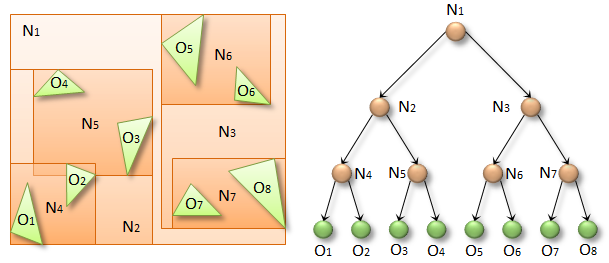
\includegraphics[width=8cm]{Figures/bvh.png}%
  \caption[Ukázka BVH stromu]{Ukázka BVH stromu~\cite{BVH}}%
  \label{fig:bvh}%
\end{figure}

\subsubsection*{Obalová struktura}
Obalová struktura může být libovolné 3D těleso, které definuje hranice objektů obsažených v obalové struktuře. Obalová struktura by měla v ideálním případě vytvořit takové těleso, které co nejtěsněji obalí objekty. Co nejpřesněji vytvořená obalová struktura se používá např. při detekci kolizí. Pro potřebu urychlení traverzace paprsku scénou je ale možné použít i jednodušší struktury. Jednou z nejčastěji používaných jednodušších struktur je struktura AABB.\par
AABB (Axis-Aligned Bounding Box) je struktura, definována dvěma body. Tyto dva body definují rohy pomyslného kvádru. Tento kvádr ve scéně definuje hranice objektů náležících tomuto objemu. Použití AABB struktury pro urychlení výpočtu traverzace paprsku je výhodné z důvodu triviálního výpočtu průniku paprsku s touto strukturou.

\subsubsection*{Tvorba BVH stromu}
Pro tvorbu BHV stromu existuje množství různých přístupů. Tvorba BVH stromu v zásadě probíhá rekurzivním dělením prostoru podle nějaké metriky. Prostor je definován obalovou strukturou, která se rekurzivně dělí tak dlouho, dokud listy BVH stromu nejsou jednotlivá tělesa.\par
Jednou z možností je dělení prostoru na poloviny jednoduchým dělením struktury na dvě části v geometrické polovině prostoru. Dělení se vždy provádí pouze v jedné ose. Osa pro dělení je zvolena ta, ve které je velikost aktuální obalové struktury maximální. Tato metoda není příliš efektivní, jelikož může jednoduše nastat situace, kdy není BVH strom vyvážený. Průchod nevyváženým stromem pak není efektivní.\par
Další z možností je dělení prostoru na poloviny takovým způsobem, aby v každé ze dvou částí byl stejný počet objektů. Tímto je vyřešen nedostatek primitivního dělení. V takovém případě se tělesa v aktuálně prohledávané obalové struktuře seřadí do pole podle pozice a vybere se těleso v polovině pole. Následně se vytvoří dvě nové obalové struktury, každá obsahující tělesa z jedné poloviny pole.\par
Jedním z aktuálně nejpoužívanějších způsobů pro dělení obalové struktury je metoda SAH (Surface Area Heuristic). Tato metoda používá jako svou metriku minimalizaci obsahů jednotlivých podstromů. To znamená, že při použití SAH je součet obsahů dvou nově vytvořených obalových struktur v aktuální obalové struktuře minimální. Při použití této metody je při dělení potřeba několikrát rozdělit obalovou strukturu a porovnat jednotlivé možnosti. Z tohoto důvodu je tvorba BVH stromu s použitím SAH výpočetně náročnější než první dvě možnosti. Díky kvalitnějšímu rozdělení prostoru je ale použití SAH výhodnější. V porovnání s první a druhou popisovanou metodou je traverzace při použití SAH až 2\(\times\) rychlejší~\cite{SAH}. Metoda SAH je ve výchozím stavu použita při tvorbě scény za pomocí knihovny Embree.

\subsection{Kd-tree}
Kd-tree je metoda pro dělení prostoru pomocí tzv. BSP (Binary Space Partitioning). Kd-tree dělí prostor na oblasti, které nemusí mít stejnou velikost. Zároveň lze dělení provést podél libovolného směru, směr nemusí být rovnoběžný s osou souřadného systému. Tato vlastnost ale může být pro potřeby urychlení traverzace paprsku kontraproduktivní. Proto je vhodnější při použití Kd-tree vždy dělit prostor podél jedné z os souřadného systému.\par
Stejně jako BVH strom je Kd-tree reprezentován binárním stromem. Na rozdíl od BVH, v Kd-tree se může objekt vyskytovat vícekrát. Jednotlivé obalové struktury se tak mohou překrývat.\par
Alternativní variantou je dále datová struktura Octree. Octree je v zásadě Kd-tree, který však nepoužívá pro dělení jeden řez, ale tři řezy. To znamená, že každý list stromové struktury má osm potomků. Hlavní výhodou použití Octree místo Kd-tree je jednodušší a rychlejší vkládání nových prvků.\par
Při tvorbě Kd-tree i Octree lze použít při dělení stejné metriky, jako u BVH. Na rozdíl od BVH je však metrika SAH upravena. V tomto případě SAH metrika upřednostňuje řez, při kterém vznikne potomek, který je zároveň list.


\section{Optimalizace vzorkování}
Jak již bylo demonstrováno dříve na praktickém příkladu v \hyperref[sec:samplingViz]{kapitole~\ref{sec:samplingViz}}, je vhodné kombinovat zvolenou BRDF funkci s funkcí pro vzorkování. Následující kapitoly se zabývají rozborem vzorkovacích funkcí, které lze použít v kombinaci s BRDF funkcemi popisovanými v této práci.

\subsection{Vzorkování hemisféry} \label{sec:hemisphere}
Jednou z nejjednodušších metod pro vzorkování je vzorkování hemisféry. Uniformní vzorkování hemisféry je definováno \hyperref[eq:hemisphereSampling]{vzorcem~\ref{eq:hemisphereSampling}} (ve sférických souřadnicích). Rozdělení pravděpodobnosti je konstantní, definováno \hyperref[eq:hemisphereSamplingPdf]{vzorcem~\ref{eq:hemisphereSamplingPdf}}. Při tomto vzorkování jsou všechny paprsky rovnoměrně rozdělené, všechny směry mají stejnou pravděpodobnost odrazu. Takové vzorkování je možné použít pro všechny BRDF funkce. Nevýhodou tohoto vzorkování je ale neoptimálnost vůči různým BRDF funkcím. Ideálně by vzorkovací funkce měla co nejpřesněji kopírovat BRDF funkci.\par

\begin{eqnarray}
  \theta & = & \arccos(\randU) \nonumber \\
  \phi & = & 2\pi\randV \label{eq:hemisphereSampling}
\end{eqnarray}

\begin{equation} \label{eq:hemisphereSamplingPdf}
  p = \frac{1}{2\pi}
\end{equation}

Jedna z možností optimalizace je použití vzorkování hemisféry závislého na cosinu úhlu mezi vstupním paprskem a normálou povrchu. Základní tezí je, že paprsky s největším úhlem mají nejmenší vliv na výsledné osvětlení v daném bodě. Vzorkování by tedy mělo mít rozložení vzorků více kumulované ve směru normály oproti ostatním směrům. Jednou z možností, jak generovat paprsky touto metodou je pomocí Malleyho metody. Tato metoda spočívá v generování bodu v jednotkovém disku pomocí soustředných kruhů~\cite{PHARR2017747}. Výsledné souřadnice v kartézském systému se vypočítají pomocí \hyperref[eq:concentricHemisphere]{vzorce~\ref{eq:concentricHemisphere}}. Pro výpočet je potřeba převést \(\randU\) a \(\randV\) z intervalu \(\intervalco{0}{1}\) do intervalu \(\intervalco{-1}{1}\)  Rozdělení pravděpodobnosti je definováno \hyperref[eq:concentricHemisphere]{vzorcem~\ref{eq:concentricHemispherePdf}}.

\begin{eqnarray}
  r & = & \left\{\begin{matrix*}[l] \randU & |\randU| > \left | \randV \right |\\ \randV & jinak \end{matrix*}\right. \nonumber \\
  \Theta & = & \left\{\begin{matrix*}[l] \frac{\pi}{4}\frac{\randV}{\randU} & |\randU| > \left | \randV \right |\\ \frac{\pi}{2}-\frac{\pi}{4}\frac{\randU}{\randV} & jinak \end{matrix*}\right. \nonumber \\
  x & = &r\cos(\Theta)\nonumber \\
  y & = &r\sin(\Theta)\nonumber \\
  z & = &\sqrt{ \max(0, 1 - x^2 + y^2) }\label{eq:concentricHemisphere}
\end{eqnarray}

\begin{equation} \label{eq:concentricHemispherePdf}
  p = \frac{\cos\theta}{\pi}
\end{equation}

\subsection{Vzorkování BRDF podle Phongova modelu} \label{sec:phongSampling}
Pro vzorkování BRDF podle Phongova modelu je potřeba rozhodnout, kterou část BRDF vzorkujeme -- jestli difuzivní nebo odrazovou. Toto rozhodnutí je možné vytvořit náhodně, pomocí vygenerování náhodného čísla \(\xi\) z intervalu \(\intervalcc{0}{k_d+k_s}\). Pokud \(\xi < k_d\), je vzorkována difuzivní část. V opačném případě je vzorkována odrazová část~\cite{KrivanekBRDFIBL}.
\subsection{Vzorkování difuzivní části}
Difuzivní část je možné vzorkovat pomocí \hyperref[sec:hemisphere]{hemisféry (\ref{sec:hemisphere})}. Je možné také použít hemisféru závislou na cosinu úhlu mezi vstupním paprskem a normálou povrchu.

\subsubsection*{Vzorkování odrazové části}
Pro vzorkování odrazové části je vzorkován Phongův cosinový lalok, který je vycentrován okolo \(\refl\). Výpočet vzorkování odrazové části je definován \hyperref[eq:phongSpecularSample]{vzorcem~\ref{eq:phongSpecularSample}}~\cite{KrivanekBRDFIBL}. Rozdělení pravděpodobnosti je definováno \hyperref[eq:phongSpecularSamplePdf]{vzorcem~\ref{eq:phongSpecularSamplePdf}}.
Výsledek tohoto vzorkování je vycentrován okolo normály, je tedy potřeba rotovat výsledek podél \(\refl\). K rotaci vektoru je možné využít \hyperref[eq:vectRotationSimple]{vzorec~\ref{eq:vectRotationSimple}}.

\begin{eqnarray}
  \theta & = & \arccos(\randU^{\frac{1}{n+1}}) \nonumber \\
  \phi & = & 2\pi\randV\label{eq:phongSpecularSample}
\end{eqnarray}

\begin{equation} \label{eq:phongSpecularSamplePdf}
  p = \frac{n+1}{2\pi}\cos^n\theta
\end{equation}

\subsubsection*{Výsledné vzorkování}
Po spojení vzorkování odrazové a difuzivní části je vhodné adaptovat i výpočet samotného BRDF\@. Při vzorkování difuzivní části je třeba jako BRDF funkci použít pouze difuzivní část BRDF podle Phongova modelu, při vzorkování odrazové části je použita odrazová část BRDF podle Phongova modelu\@. Pokud by se použilo BRDF podle Phongova modelu bez úpravy, nebylo by dosaženo snížení variance ve výsledném obrazu.~\cite{KrivanekBRDFIBL}

\subsection{Vzorkování světelných zdrojů z HDR mapy}
Pro vzorkování z HDR mapy je potřeba nejprve určit metodiku vzorkování z diskrétní 2D veličiny. Je možné interpretovat 2D veličinu jako 1D veličinu, ale takový přístup není optimální. Lepší řešení je přijít se vzorkováním, které vzorkuje 2D veličinu pomocí dvou náhodných čísel, pomocí dvou marginálních distribucí. V takovém případě je možné vzorkovat z 2D veličiny jako z matice. Nejprve je potřeba vypočítat marginální distribuce. Je možné počítat distribuce ve sloupcích nebo v řádcích. V případě výpočtu marginálních distribucí ve sloupcích je potom vzorkován řádek z daného sloupce, v opačném případě je vzorkován sloupec z daného řádku. Pomocí hodnot \(\randU\) a \(\randV\) je vybrána distribuce, resp.\ výsledná vzorkovaná hodnota.~\cite{PHARR2017747}\par
Tento postup je vhodný provádět na obrazových datech, na kterých je sníženo rozlišení. Díky snížení rozlišení se zjednoduší výpočet a spojí se větší světelné zdroje do jedné oblasti.


\begin{figure}[ht]%
  \centering
  \subfloat[HDR mapa]{{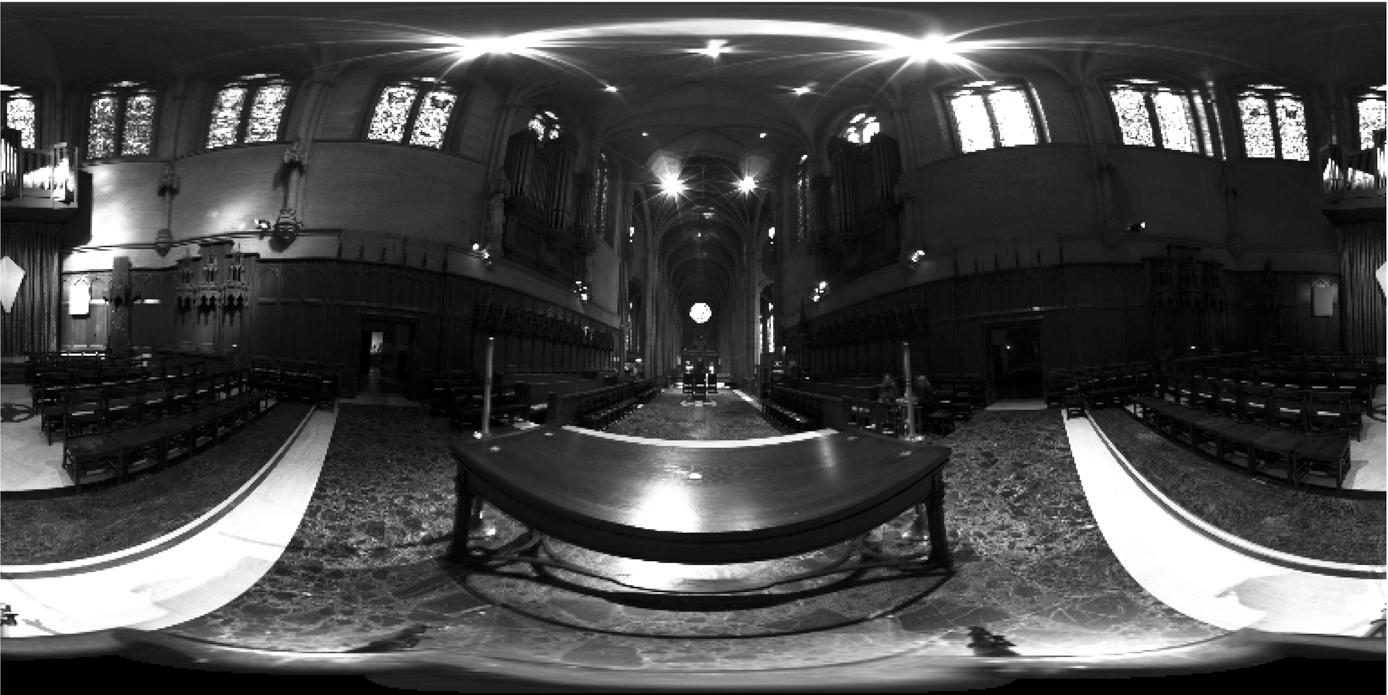
\includegraphics[width=6cm]{Figures/hdr-env-orig.png} }}%
  \qquad
  \subfloat[HDR mapa s marginální distribucí]{{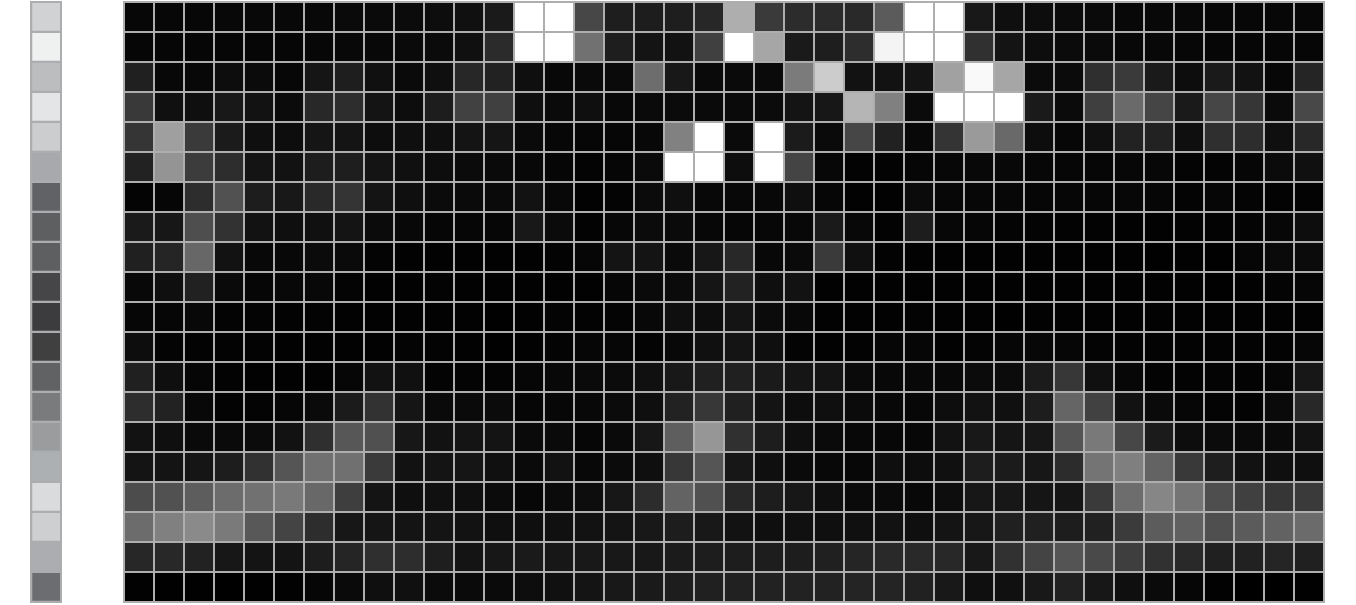
\includegraphics[width=6cm]{Figures/hdr-env-marginal-conditional.png} }}%
  \caption[Postup vzorkování světelných zdrojů]{Postup vzorkování světelných zdrojů~\cite{PHARR2017747}}%
  \label{fig:lightsSampling}%
\end{figure}

\subsection{Multiple importance sampling}
Jednotlivé, samostatné možnosti vzorkování mají pozitivní vliv na výkon aplikace. Samostatné vzorkování pouze BRDF funkce, nebo pouze světelných zdrojů ale nedává optimální výsledky (viz \hyperref[fig:samplingBRDFOnly]{obrázek~\ref{fig:samplingBRDFOnly}} a \hyperref[fig:samplingLightsOnly]{obrázek~\ref{fig:samplingLightsOnly}}). Ve článku~\cite{Guibas1997RobustMC} je představena metoda MIS (Multiple Importance Sampling). Pomocí metody MIS lze spojit libovolný počet vzorkovacích technik. Pro výsledné vzorkování je pak použit výpočet definovaný \hyperref[eq:misEstimator]{vzorcem~\ref{eq:misEstimator}}. Pro výpočet je nutné každé vzorkovací technice přiřadit koeficient \(w\). Tento koeficient nemusí být konstantní, je možné jej dynamicky měnit podle současného vzorku. Pro všechny koeficienty \(w\) pak musí platit podmínky \hyperref[eq:weightCond1]{\ref{eq:weightCond1}} a  \hyperref[eq:weightCond2]{\ref{eq:weightCond2}}.

\begin{equation} \label{eq:misEstimator}
  F = \sum^{n}_{i=1}\frac{1}{n_i}\sum^{n_i}_{j=1}w_i(X_{i,j})\frac{f(X_{i,j})}{p_i(X_{i,j})}
\end{equation}

\begin{align}
  \sum^{n}_{i=1}w_i(x) & = 1 \text{~pro~}f\left( x \right) \neq 0 \label{eq:weightCond1} \\
  w_i\left( x \right)  & = 0 \text{~pro~}p_i\left( x \right) = 0 \label{eq:weightCond2}
\end{align}

Pro získání koeficientů \(w\) je ve článku~\cite{Guibas1997RobustMC} navržena dvojice heuristik, která je definovaná \hyperref[eq:balancePowerHeuristic]{vzorcem~\ref{eq:balancePowerHeuristic}}. Jedná se o tzv. \textquote{balance heuristic} a \textquote{power heuristic}. Tato dvojice heuristik patří aktuálně mezi jedny z nejpoužívanějších.\par
O balance heuristic -- vyváženou heuristiku se jedná v případě, kdy \(\beta = 1\). Ve článku~\cite{Guibas1997RobustMC} je tvrzení, že žádná jiná heuristika (v té době) neměla výrazně lepší výsledky než právě tato heuristika. V případě, že \(\beta > 1\), jedná se o Power heuristic. Tato heuristika je vhodná pro aplikace s obecně menší variancí. Parametr \(\beta\) je možné nastavit libovolně, experimentálně, ve článku~\cite{Guibas1997RobustMC} je navrženo nastavení \(\beta = 2\). Výsledek použití metody MIS s Balance heuristikou je zobrazen na \hyperref[fig:samplingMIS]{obrázku~\ref{fig:samplingMIS}}

\begin{equation} \label{eq:balancePowerHeuristic}
  w_i\left( x \right) = \frac{\left[n_{i} p_{i}(x)\right]^\beta}{\sum_{k}\left[n_kp_k(x)\right]^\beta}
\end{equation}

Balance a Power heuristika nabízí robustní kombinaci vzorkování, kdy i při horší kombinaci vstupů není negativně ovlivněn celkový výstup. Nevýhodou ale je horší efektivita tohoto přístupu. V některých případech může např.\ dojít k situaci, kdy by lepšího výsledku bylo dosaženou použitím pouze jedné vzorkovací techniky. Tento problém a jeho následné řešení byl podrobně popsán v článku~\cite{OptimalMIS}. Výpočet heuristiky je popsán \hyperref[eq:misOptimalWeighs]{vzorcem~\ref{eq:misOptimalWeighs}}. Heuristika pro svůj výpočet používá dodatečný parametr \(\alpha\), který lze získat pomocí řešení \hyperref[eq:misOptimalWeighsAlpha]{lineárního systému~\ref{eq:misOptimalWeighsAlpha}}. Pro výpočet je nutná matice hodnot \(a\) a vektor hodnot \(b\). Tyto hodnoty jsou získány pomocí \hyperref[eq:misOptimalWeighsAB]{rovnic~\ref{eq:misOptimalWeighsAB}}.

\begin{equation} \label{eq:misOptimalWeighs}
  w_i\left( x \right) = \frac{\alpha_i p_i\left( x \right)}{f\left( x \right)} + \frac{n_i p_i(x)}{\sum^{N}_{k=1}n_k p_k(x)}\left(1-\frac{\sum^{N}_{k=1}\alpha_k p_k\left( x \right)}{f(x)}\right)
\end{equation}

\begin{equation} \label{eq:misOptimalWeighsAlpha}
  \begin{pmatrix} a_{11} & \cdots & a_{1N} \\ \vdots & \ddots & \vdots \\ a_{N1} & \cdots & a_{NN} \end{pmatrix} \begin{pmatrix} \alpha_{1} \\ \vdots \\ \alpha_{N} \end{pmatrix} = \begin{pmatrix} b_{1} \\ \vdots \\ b_{N} \end{pmatrix}
\end{equation}

\begin{align} \label{eq:misOptimalWeighsAB}
  a_{ij} & = \int\frac{p_i p_j}{\sum^{N}_{k=1}n_k p_k} \\
  b_{i}  & = \int\frac{p_i f}{\sum^{N}_{k=1}n_k p_k}
\end{align}

\begin{figure}[ht]%
  \centering
  \subfloat[Vzorkování BRDF\label{fig:samplingBRDFOnly}]{{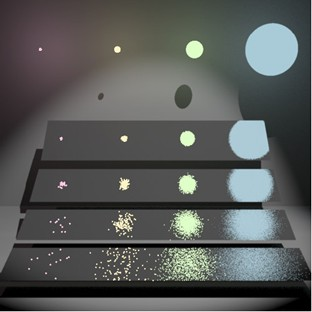
\includegraphics[width=6cm]{Figures/brdfsampling.jpg} }}%
  \qquad
  \subfloat[Vzorkování světelných zdrojů\label{fig:samplingLightsOnly}]{{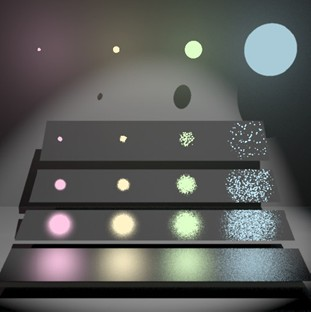
\includegraphics[width=6cm]{Figures/lightsampling.jpg}}}%
  \qquad
  \subfloat[Multiple importance sampling\label{fig:samplingMIS}]{{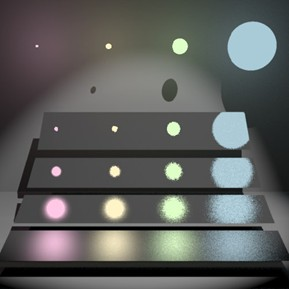
\includegraphics[width=6cm]{Figures/mis.jpg} }}%
  \caption[Srovnání výsledků vzorkování]{Srovnání výsledků vzorkování~\cite{Guibas1997RobustMC}}%
  \label{fig:samplingComparison}%
\end{figure}


\chapter{Závěr}
Byla vytvořena multiplatformní aplikace v jazyce C++, která umožňuje interaktivně vizualizovat vybrané analyticky zadané BRDF funkce i s výsledným renderem. V aplikaci je také možné vizualizovat vzorkovací funkce a demonstrovat vliv výběru vzorkovacích funkcí na výsledný render. Aplikace je snadno rozšiřitelná o případné další BRDF funkce a vzorkovací funkce.\par
V první kapitole bylo sjednoceno značení veličin a parametrů BRDF funkcí, které byly používány ve vzorcích. U některých veličin byl také upřesněn výpočet, který je možné použít pro získání jejich hodnoty. U parametrů BRDF funkcí bylo také zmíněno, který parametr je pro kterou BRDF funkci relevantní. \par
Ve druhé kapitole diplomové práce byly zpracovány existující aplikace, sloužící k vizualizaci a návrhu BRDF funkcí. Popsány byly funkcionality jednotlivých aplikací, byly zmíněny zajímavé vlastnosti a nedostatky. Na konci druhé kapitoly byly popsány požadavky na implementaci aplikace, vycházející z vlastností existujících aplikací a řešící některé z nedostatků.\par
Ve třetí kapitole diplomové práce byly teoreticky popsány principy osvětlení scény společně s osvětlením pomocí HDR mapy. Byl popsán princip sledování paprsku, zobrazovací rovnice a její řešení s použitím metody Monte Carlo.\par
Ve čtvrté kapitole byl teoreticky rozebrán princip BRDF funkce, společně s podmínkami pro fyzikální přesnost. Následně byly popsány vybrané BRDF funkce. Každá BRDF funkce byla popsána analyticky, byly popsány případné parametry a také bylo uvedeno, pro které materiály se daná BRDF funkce hodí. Také byla každá BRDF funkce vizualizována pomocí snímku z vytvořené aplikace. Na konci kapitoly byl pak srovnán výkon jednotlivých BRDF funkcí za pomocí naměřených dat.\par
Pátá kapitola se věnovala popisu vytvořené aplikace. Jednotlivé části aplikace byly popsány a výsledky těchto částí byly zobrazeny. Byl rozebrán princip zobrazení BRDF funkcí, vybraného vzorkování a také výsledku path tracingu vzniklého pomocí metody path tracing. Dále byly také zpracovány důležité pomocné matematické funkce. Nakonec byly popsány použité knihovny.\par
V poslední kapitole byly rozebrány jednotlivé možnosti optimalizace metody Monte Carlo pro řešení zobrazovací rovnice. Byly teoreticky popsány akcelerační datové struktury a podrobněji bylo rozvedeno použití BVH stromu a Kd-tree. Následně byly teoreticky zpracovány možnosti optimalizace pomocí vzorkování. Bylo popsáno vzorkování samotných BRDF funkcí i vzorkování světelných zdrojů z HDR mapy. Následně bylo popsáno možné spojení těchto dvou vzorkovacích metod pomocí metody Multiple Importance Sampling.\par
\subsection*{Možná vylepšení aplikace}
Aplikace jako taková by mohla být dále rozšířena o několik různých funkcí. V aktuálním stavu je aplikace závislá na BRDF funkcích přímo implementovaných v kódu. Bylo by teda možné rozšířit aplikaci o načítání uživatelsky definovaných BRDF funkcí. Zde však vzniká problém, jelikož je potřeba definovat BRDF funkci pro GLSL shader a také pro výpočet pomocí Embree. Bylo by teda potřeba tento výpočet sjednotit. Možným řešením by bylo použití např.\ jazyka Lua pro definici BRDF funkcí a jejich parametrů. Kód by pak musel být zpracován a zkompilován za běhu aplikace pro glsl shader. Obohacující by také mohla být podpora pro načítání BRDF modelů získaných z reálně naměřených dat. Nabízelo by se tak použití např.\ dat z databáze MERL. Další možností by mohla být interaktivní úprava kódu pro BRDF funkci přímo za běhu aplikace. Funkce by mohlo být možné upravovat přímo textově, nebo by mohl být vytvořen systém pro vizuální programování. Takové systémy se stávají populární, lze je nalézt např.\ v Unreal Engine 4, nebo v Blender. Z hlediska výkonu by aplikace mohla být upravena tak, aby byl volitelný způsob výpočtu finálního renderu. Kromě výpočtu na CPU s použitím knihovny Embree by mohla být přepínatelná podpora pro výpočet na GPU např.\ pomocí technologie Vulkan, Nvidia OptiX, nebo OpenCL.

\printbibliography[title={Literatura}, heading=bibintoc]

\appendix
\chapter{Celkové srovnání všech BRDF funkcí}
\begin{table}[ht]
  \centering
  \begin{tabular}{ld{3}d{3}}
    \toprule
    BRDF Funkce              & \multicolumn{1}{r}{Absolutní čas} & \multicolumn{1}{r}{Relativní čas} \\
    \midrule
    Mirror                   & 0.04~\text{s}                     & 1.00                              \\
    Lambert                  & 0.05~\text{s}                     & 1.27                              \\
    Phong                    & 0.41~\text{s}                     & 10.84                             \\
    Physically correct Phong & 0.48~\text{s}                     & 12.79                             \\
    Blinn-Phong              & 0.50~\text{s}                     & 13.25                             \\
    Cook-Torrance            & 0.53~\text{s}                     & 13.98                             \\
    Torrance-Sparrow         & 0.54~\text{s}                     & 14.18                             \\
    Oren-Nayar               & 1.36~\text{s}                     & 36.00                             \\
    \bottomrule
  \end{tabular}
  \caption{Celkové srovnání všech BRDF funkcí}
  \label{tab:AllBRDFsComparison}
\end{table}

\end{document}